\documentclass{beamer}
\usetheme{Dresden}
\usecolortheme{dolphin}
\usefonttheme[onlymath]{serif}

%\pdfminorversion=7 % per togliere il warning delle immagini

\setbeamertemplate{navigation symbols}{} %toglie i navigation symb. basso a dx
%\setbeamertemplate{mini frames}{} % boh non fa niente
\renewcommand*{\slideentry}[6]{} % toglie i pallini in alto
\setbeamertemplate{section in toc}[ball unnumbered] % mette i bullet nella toc

%\setbeamertemplate{headline}{%
%	\begin{beamercolorbox}{section in head/foot}%
%		\vskip2pt\insertnavigation{\paperwidth}\vskip2pt%
%	\end{beamercolorbox}%
%}

\usepackage[utf8]{inputenc}
\usepackage[T1]{fontenc}
\usepackage{lmodern}
\usepackage[british]{babel}
\usepackage{amsmath}
\usepackage{amsthm}
\usepackage{graphicx}
\usepackage{xspace}
\usepackage{subfig} % affiancare figure
\usepackage{caption} % per gestire meglio le didascalie
\usepackage{pgfplots}
\pgfplotsset{compat=newest}
\pgfplotsset{plot coordinates/math parser=false}
\usepackage{booktabs} % per i filetti delle tabelle
%\usepackage{wrapfig} % a cosa mi serve?
\usepackage{appendixnumberbeamer} % numerare da 1 nell'appendice
\usepackage[separate-uncertainty=true]{siunitx} % per le unitàdi misura

\captionsetup{skip=0pt, belowskip=0pt}
\captionsetup{labelformat=empty}
\captionsetup[subfigure]{labelformat=empty}
%\captionsetup{singlelinecheck=false}
\setbeamerfont{caption}{size=\fontsize{5}{7}}
\pgfplotsset{every tick label/.append style={font=\tiny}}

\usecolortheme{orchid} % per i block
\setbeamercovered{transparent}

\newcommand{\DUMUX}{DuMu$^\text{x}$\xspace} %for convenience

\newlength{\widthconslaw}\setlength{\widthconslaw}{0.9\textwidth}
\newlength{\heightconslaw}\setlength{\heightconslaw}{0.43\textheight}
\newlength{\limiterswidth}\setlength{\limiterswidth}{0.96\textwidth}
\newlength{\limitersheight}\setlength{\limitersheight}{0.65\textheight}
\newlength{\tvdwidth}\setlength{\tvdwidth}{0.9\textwidth}
\newlength{\tvdheight}\setlength{\tvdheight}{0.5\textheight}
\newlength{\figwidth}\setlength{\figwidth}{0.4\textwidth}
\newlength{\roughwidth}\setlength{\roughwidth}{0.9\textwidth}
\newlength{\roughheight}\setlength{\roughheight}{0.9\textheight}
\newlength{\bfswidth}\setlength{\bfswidth}{0.95\textwidth}
\newlength{\bfsheight}\setlength{\bfsheight}{0.8\textheight}
\newlength{\bfshalfwidth}\setlength{\bfshalfwidth}{0.5\textwidth}
\newlength{\cavheight}\setlength{\cavheight}{0.7\textheight}
\newlength{\timewidth}\setlength{\timewidth}{0.65\textwidth}
\newlength{\timeheight}\setlength{\timeheight}{0.65\textheight}
\newlength{\timehalfwidth}\setlength{\timehalfwidth}{0.45\textwidth}
\newlength{\timehalfheight}\setlength{\timehalfheight}{0.82\textheight}
\newlength{\widthsette}\setlength{\widthsette}{0.4\textwidth}

\graphicspath{{../img/}}

%%%%%%%%%%%%%%%%%%%
% per la numerazione delle slides
\newcommand{\frameofframes}{/}
\newcommand{\setframeofframes}[1]{\renewcommand{\frameofframes}{#1}}

\setframeofframes{of}
\makeatletter
\setbeamertemplate{footline}
{%
	\begin{beamercolorbox}[colsep=1.5pt]{upper separation line foot}
	\end{beamercolorbox}
	\begin{beamercolorbox}[ht=2.5ex,dp=1.125ex,%
		leftskip=.3cm,rightskip=.3cm plus1fil]{author in head/foot}%
		\leavevmode{\usebeamerfont{author in head/foot}\insertshortauthor}%
		\hfill%
		{\usebeamerfont{institute in head/foot}\usebeamercolor[fg]{institute in 
		head/foot}\insertshortinstitute}%
	\end{beamercolorbox}%
	\begin{beamercolorbox}[ht=2.5ex,dp=1.125ex,%
		leftskip=.3cm,rightskip=.3cm plus1fil]{title in head/foot}%
		{\usebeamerfont{title in head/foot}\insertshorttitle}%
		\hfill%
		{\usebeamerfont{frame number}\usebeamercolor[fg]{frame 
		number}\insertframenumber~\frameofframes~\inserttotalframenumber}
	\end{beamercolorbox}%
	\begin{beamercolorbox}[colsep=1.5pt]{lower separation line foot}
	\end{beamercolorbox}
}
\makeatother
%%%%%%%%%%%%%%%%%%%%%%%%%%%%%%%%%
\title{A fully implicit formulation for Navier-Stokes/Darcy coupling}
\author[Andrea Vescovini]{Andrea Vescovini\texorpdfstring{\\[2.5ex]\scriptsize%
%		\parbox{2cm}{Supervisor:\\Co-Supervisors:\\~}\hspace{0.1cm}\parbox{4cm}{Prof. Luca Formaggia\\Dr. Anna Scotti\\Prof. Dr.-Ing. Rainer Helmig}}%
%Supervisor: Prof. Luca Formaggia\\[0.5ex]Co-supervisors: Dr. Anna Scotti and Prof. Dr.-Ing. Rainer Helmig}%
\begin{tabular}{ll}
	Supervisor: & Prof. Luca Formaggia\\
	Co-supervisors: & Dr. Anna Scotti\\
	& Prof. Dr.-Ing. Rainer Helmig\\
\end{tabular}}
{Supervisor: Prof. Luca Formaggia}}

\institute[Politecnico di Milano - Universit\"at Stuttgart]%
		  {Politecnico di Milano - Universit\"at Stuttgart}%\\%
%[2ex]
\includegraphics[height=1cm, keepaspectratio]{logopoli.png}\hspace{1cm}%
%	 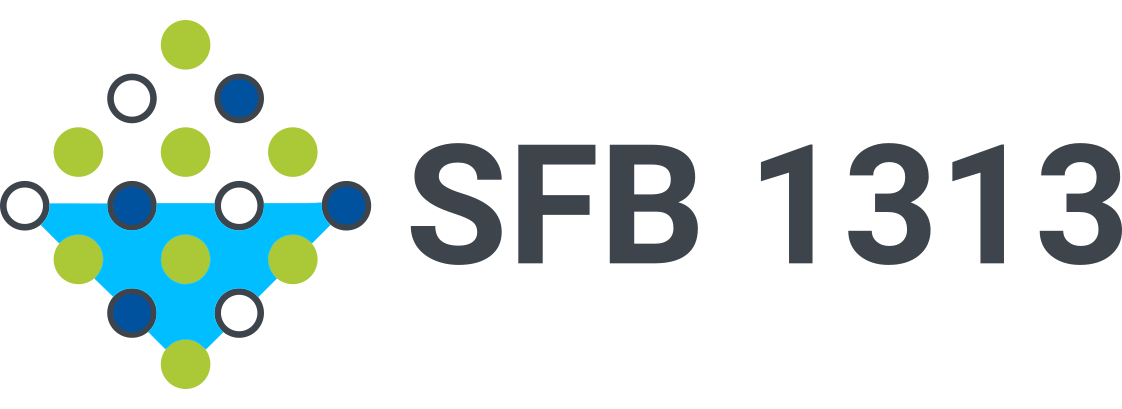
\includegraphics[height=1cm, keepaspectratio]{logosfb.png}\hspace{1cm}%
%	 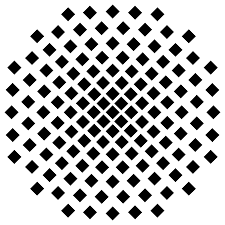
\includegraphics[height=1cm, keepaspectratio]{logostutt.png}}
\date{16th April 2019}
%%%%%%%%%%%%%%%%%%%%%%%%%%%%%%%%%%%%%%%%%%%%%%%%%%%%%%%%%%%%%%%%%%%%%%%%%%%%
\begin{document}
\begin{frame}
	\vspace{0.3cm}
	\centering
	
\includegraphics[height=0.9cm, 
	keepaspectratio]{logopoliblu.png}\hspace{0.5cm}%
	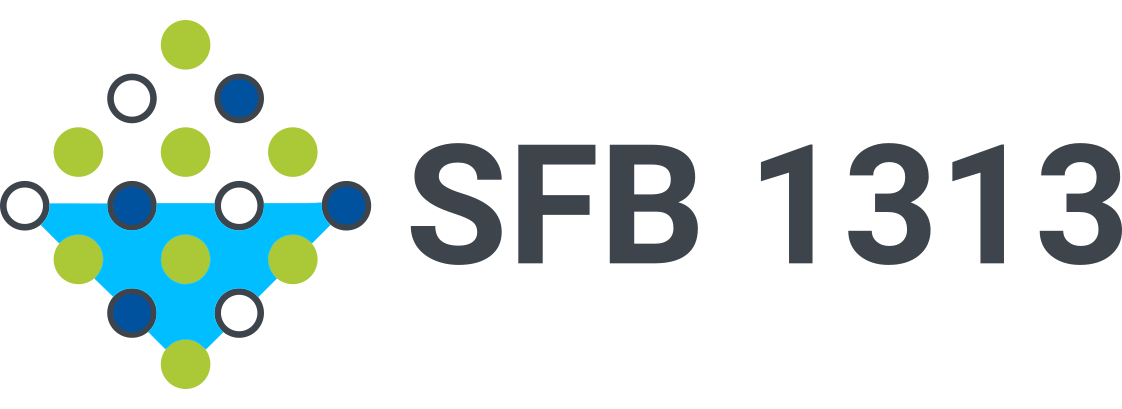
\includegraphics[height=0.9cm, keepaspectratio]{logosfb.png}\hspace{0.5cm}%
	
\includegraphics[height=0.9cm, keepaspectratio]{logostuttnome.png}
	\vspace{0.3cm}
	\setlength\tabcolsep{3pt} % default value: 6pt
	\maketitle
	\setlength\tabcolsep{6pt} % default value: 6pt
\end{frame}
%%%%%%%%%%%%%%%%%%%%%%%%%%%%%%%%%%%%%%%%%%%%%%%%%%%%%%%%%%%%%%%%%%%%%%%%%%%%
\begin{frame}{Introduction}
Coupled \textbf{free-flow} and \textbf{porous-medium flow} systems involve 
complex phenomena acting at different scales:
\begin{figure}
	\centering
	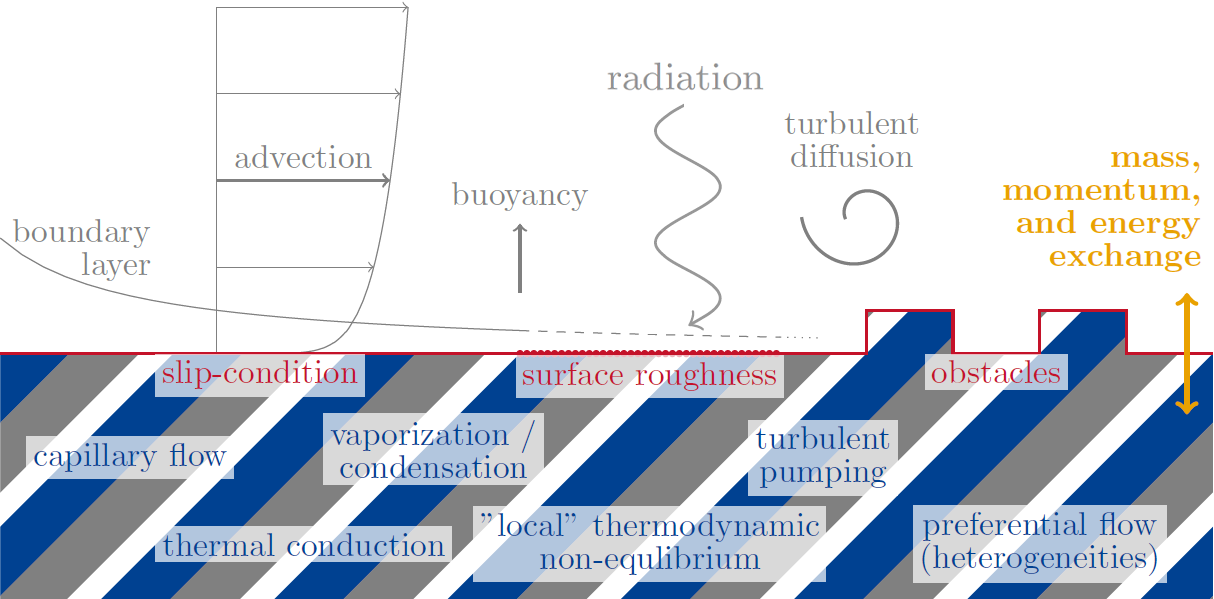
\includegraphics[width=0.8\textwidth]{intropicture2.png}
	\caption{\color{gray}T. Fetzer. Coupled Free and Porous-Medium Flow 
	Processes Affected by Turbulence and Roughness.}
\end{figure}
Applications: soil salinization, PEM fuel cells, drying processes, etc.
\end{frame}
%%%%%%%%%%%%%%%%%%%%%%%%%%%%%%%%%%%%%%%%%%%%%%%%%%%%%%%%%%%%%%%%%%%%%%%%%%%%
%\begin{frame}{Introduction}
%Several analysis can be found in literature:
%\begin{itemize}
%	\item single-domain or two-domain approach.
%	\item coupling concepts for different levels of complexity.
%	\item monolithic or iterative solution procedures.
%	\item turbulence and roughness effects.
%\end{itemize}
%%\pause
%\vspace{0.5cm}
%Considering a \textbf{single-phase}, \textbf{single-component}, 
%\textbf{isothermal fluid}, the aims of this thesis are:
%\begin{itemize}
%	\item to implement and test \textbf{TVD methods} for the free-flow model.
%	\item to study the effect of \textbf{rough interfaces} between the two 
%	subdomains of a coupled model.
%\end{itemize}
%\end{frame}
%
\begin{frame}{Introduction}
We consider a \textbf{single-phase}, \textbf{single-component}, 
\textbf{isothermal fluid}, in \textbf{turbulent conditions}.\\
\vspace{0.3cm}
We want to study the effect on the flow field of \textbf{rough interfaces} 
between the two 
subdomains of a coupled model:
\begin{itemize}
	\item it is an unavoidable aspect in natural systems.
	\item few results can be found in literature.
\end{itemize}
\vspace{0.3cm}
We implemented \textbf{TVD methods} for the free-flow model within the 
C++ library \DUMUX:
\begin{itemize}
	\item an accurate free-flow model in important especially in turbulent 
	conditions.
	\item it is important to have a robust method.
\end{itemize}
\end{frame}
%%%%%%%%%%%%%%%%%%%%%%%%%%%%%%%%%%%%%%%%%%%%%%%%%%%%%%%%%%%%%%%%%%%%%%%%%%%%
\begin{frame}{Outline}
	\tableofcontents
\end{frame}
%%%%%%%%%%%%%%%%%%%%%%%%%%%%%%%%%%%%%%%%%%%%%%%%%%%%%%%%%%%%%%%%%%%%%%%%%%%%
\section{Governing equations}
\begin{frame}{Free-flow}
Incompressible RANS equations:
\begin{align*}
\nabla \cdot \bar{\mathbf{v}} = 0&\\
\frac{\partial \bar{\mathbf{v}}}{\partial t} + \nabla 
\cdot (\bar{\mathbf{v}} \bar{\mathbf{v}}^\mathrm{T}) - \nabla \cdot 
((\nu + \nu_t) \nabla \bar{\mathbf{v}}) + \frac{1}{\varrho}\nabla (p + \frac{2}{3}\varrho k) = \mathbf{0}&
\end{align*}
$k\text{-}\omega$ turbulence model $\nu_t = k / \tilde{\omega}$ with limiters:
\begin{align*}
&\frac{\partial k}{\partial t} + \nabla \cdot (k\bar{\mathbf{v}}) - \nabla \cdot
\bigg[\bigg(\nu + \sigma^*\frac{k}{\omega}\bigg) \nabla k\bigg] -P + \beta^* k 
\omega = 0\\
%\end{gather*}
%\begin{multline*}
&\frac{\partial \omega}{\partial t} + \nabla \cdot (\omega \bar{\mathbf{v}}) - 
\nabla \cdot \bigg[ \bigg( \nu + \sigma \frac{k}{\omega} \bigg) \nabla \omega 
\bigg]-\\
&\hspace{2.5cm}- \alpha \frac{\omega}{k} 2 \nu_t \bar{\mathbf{S}} \cdot \bar{\mathbf{S}} 
-\frac{\sigma_d}{\omega} \nabla k \cdot 
\nabla \omega+ \beta \omega^2 = 0
\end{align*}
\end{frame}
%%%%%%%%%%%%%%%%%%%%%%%%%%%%%%%%%%%%%%%%%%%%%%%%%%%%%%%%%%%%%%%%%%%%%%%%%%
\begin{frame}{Porous-medium flow - REV scale approach}
Continuity equation for a single-phase incompressible fluid:
\begin{equation*}
\nabla \cdot \mathbf{v} = 0
\end{equation*}
Momentum equation:
\begin{itemize}
	\item Darcy's law:
\begin{equation*}
	\mathbf{v} = -\frac{1}{\mu}\mathbf{K} \nabla p
\end{equation*}
	\item Forchheimer's law:
	\begin{equation*}
	\mathbf{v} + C_F \sqrt{\mathbf{K}} \frac{\varrho}{\mu} |\mathbf{v}| 
	\mathbf{v} = - \frac{1}{\mu}\mathbf{K} \nabla p
	\end{equation*}
	It models a quadratic drag and it holds at \textbf{higher} 
	$\boldsymbol{Re}$ than the Darcy's law.
\end{itemize}
\end{frame}
%%%%%%%%%%%%%%%%%%%%%%%%%%%%%%%%%%%%%%%%%%%%%%%%%%%%%%%%%%%%%%%%%%%%%%%%%
\begin{frame}{Coupling conditions}
%At the interface we apply:
\begin{itemize}
	\item Continuity of normal velocity:
	\begin{equation*}
	[\mathbf{v} \cdot \mathbf{n}]_\text{ff} = - [\mathbf{v} 
	\cdot \mathbf{n}]_\text{pm}
	\end{equation*}
	\item Continuity of normal stresses:
	\begin{equation*}
	[(\varrho \mathbf{v} \mathbf{v}^\mathrm{T} - (\mu + \mu_t) \nabla 
	\mathbf{v} + p\mathbf{I}) 
	\mathbf{n}]_\text{ff} = 
	- [p\mathbf{n}]_\text{pm}
	\end{equation*}
	\item Beavers-Joseph-Saffman condition for the tangential component of 
	momentum:
	\begin{equation*}
	\bigg[ \bigg( -\frac{\sqrt{\mathrm{K}}}{\alpha_\text{BJ}} (\nabla \mathbf{v}) 
	\mathbf{n} - \mathbf{v} \bigg) \cdot \mathbf{t}_i \bigg]_\text{ff} = 0 
	\quad \forall i \in \{1, \dots, dim - 1\}
	\end{equation*}
\end{itemize}
\begin{tikzpicture}[remember picture,overlay]
\node[xshift=-2cm,yshift=-1.8cm] at (current page.north east){%
	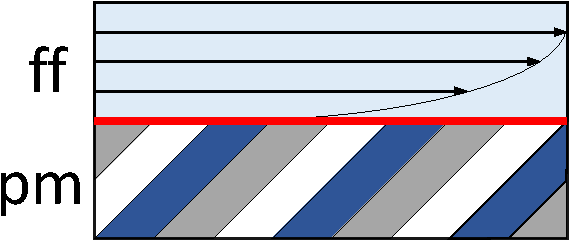
\includegraphics[width=3cm]{bjs.pdf}};
\end{tikzpicture}
\end{frame}
%%%%%%%%%%%%%%%%%%%%%%%%%%%%%%%%%%%%%%%%%%%%%%%%%%%%%%%%%%%%%%%%%%%%%%%%%%
\section{Numerical model}
\begin{frame}{Finite volumes discretization}
	\begin{itemize}
	\item \textbf{Staggered grid} approach in the free-flow:
	\begin{minipage}{0.5\textwidth}%
		\begin{figure}
			\vspace{0.1cm}
			\centering
			\includegraphics[%
			%trim={2cm 1cm 0cm 0cm}, clip, height=0.65\textheight]%
			%			trim={2cm 5.2cm 0cm 0.8cm}, clip, height=0.4\textheight]%
			trim={2cm 5.2cm 7cm 0.8cm}, clip, height=0.4\textheight]%
			{staggered_grid_mia.pdf}
			\vspace{0.2cm}
		\end{figure}
	\end{minipage}%
	\begin{minipage}{0.5\textwidth}
		\centering
		Scalar primary variables:\\
		$p$, $k$, $\omega$\\
		Vectorial primary variables:\\
		$\mathbf{v}=[u,v]^\mathrm{T}$
	\end{minipage}
	\item \textbf{Cell-centred} approach in the porous-medium flow:
	\begin{minipage}{0.5\textwidth}%
		\begin{figure}
			\vspace{0.1cm}
			%			\centering
			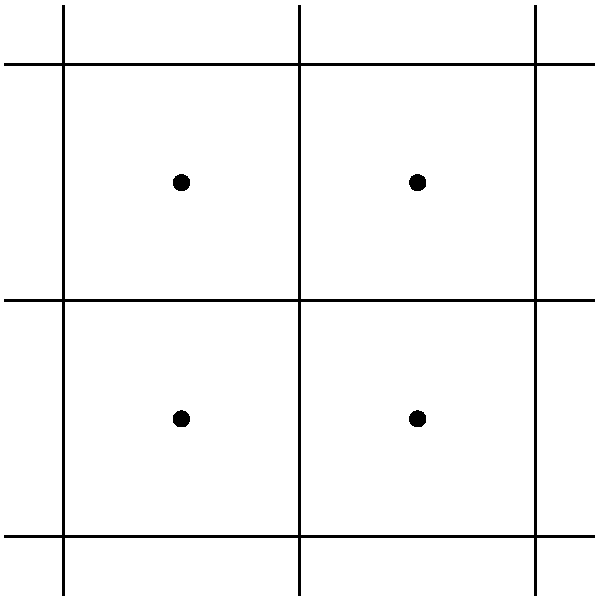
\includegraphics[height=0.3\textheight]{cellcentred.pdf}
			%			\hspace{2cm}
		\end{figure}
	\end{minipage}%
	\begin{minipage}{0.5\textwidth}
		\centering
		Scalar primary variables:\\
		$p$
	\end{minipage}%
\end{itemize}
\end{frame}
%%%%%%%%%%%%%%%%%%%%%%%%%%%%%%%%%%%%%%%%%%%%%%%%%%%%%%%%%%%%%%%%%%%%%%%%%
\begin{frame}{Differencing schemes}
Non-linear convective term of the Navier-Stokes equations:
\begin{equation*}
\int_V \nabla \cdot (\mathbf{v} \mathbf{v}^\mathrm{T}) \; dV = \int_{\partial 
V} 
\overbrace{\mathbf{v}}^{\substack{\text{\makebox[0pt]{transported}} 
		\\ \text{\makebox[0pt]{field}}}} \underbrace{(\mathbf{v} \cdot 
	\mathbf{n})}_{\substack{\text{\makebox[0pt]{transporting}} \\
		\text{\makebox[0pt]{velocity}}}} \; dA
\end{equation*}
Differencing scheme needed to approximate the transported field:
\begin{itemize}
	\item Upwind $\rightarrow$ $1^\text{st}$ order, stable, high numerical dissipation.
	\item LUD, QUICK, etc. $\rightarrow$ $2^\text{nd}$ or $3^\text{rd}$ order, unphysical oscillations.
	\item \textbf{TVD methods $\rightarrow$ 2$^\text{nd}$ order, non-linear, 
	oscillation-free}.\\
	\emph{Flux limiters: Van Leer, Min-Mod, Van Alabada, etc.}
\end{itemize}
\end{frame}
%%%%%%%%%%%%%%%%%%%%%%
%\begin{frame}{TVD methods}
%	immagine, formula
%\end{frame}
%%%%%%%%%%%%%%%%%%%%%%%%%%%%%%%%%%%%%%%%%%%%%%%%%%%%%%%%%%%%%%%%%%%%%
\begin{frame}{Resulting equations}
\begin{itemize}
\item After having performed the spatial discretization, we obtain a system of 
ODEs, which is solved using \textbf{implicit unconditionally stable} methods 
(BDF2 or Backward Euler).
\vspace{0.5cm}

\item The resulting non-linear algebraic system is solved 
\textbf{monolithically}, 
employing the \textbf{Newton's method}. The entries of the Jacobian matrix are 
computed numerically using finite differences.
\vspace{0.5cm}

\item Eventually, the linear system is solved directly using the library 
UMFPACK.
\end{itemize}
\end{frame}
%%%%%%%%%%%%%%%%%%%%%%%%%%%%%%%%%%%%%%%%%%%%%%%%%%%%%%%%%%%%%%%%%%%%%%%%
\section{Numerical results}
\begin{frame}{Free-flow validation tests}
\begin{itemize}
	\item Convergence tests refining the grid, using Navier-Stokes problems 
	with analytical solution.
	\vspace{-0.3cm}
	\begin{table}\scriptsize
		\[
		\begin{array}{c|ccc}
		\toprule
		& \text{Upwind} & \text{Min-Mod} & \text{Van Leer} \\ 
		\midrule
		p & 1.148 & 1.659 & 1.058\\
		u & 1.071 & 1.441 & 1.437\\
		v & 1.068 & 1.533 & 1.560\\
		\bottomrule
		\end{array}
		\]
%		\caption{\tiny Convergence orders with $Re = 1000$}
	\end{table}
	\item Backward facing step test: comparison with the NASA CFL3D code, at 
	$Re_H=36000$.
	\begin{figure}
		\centering
		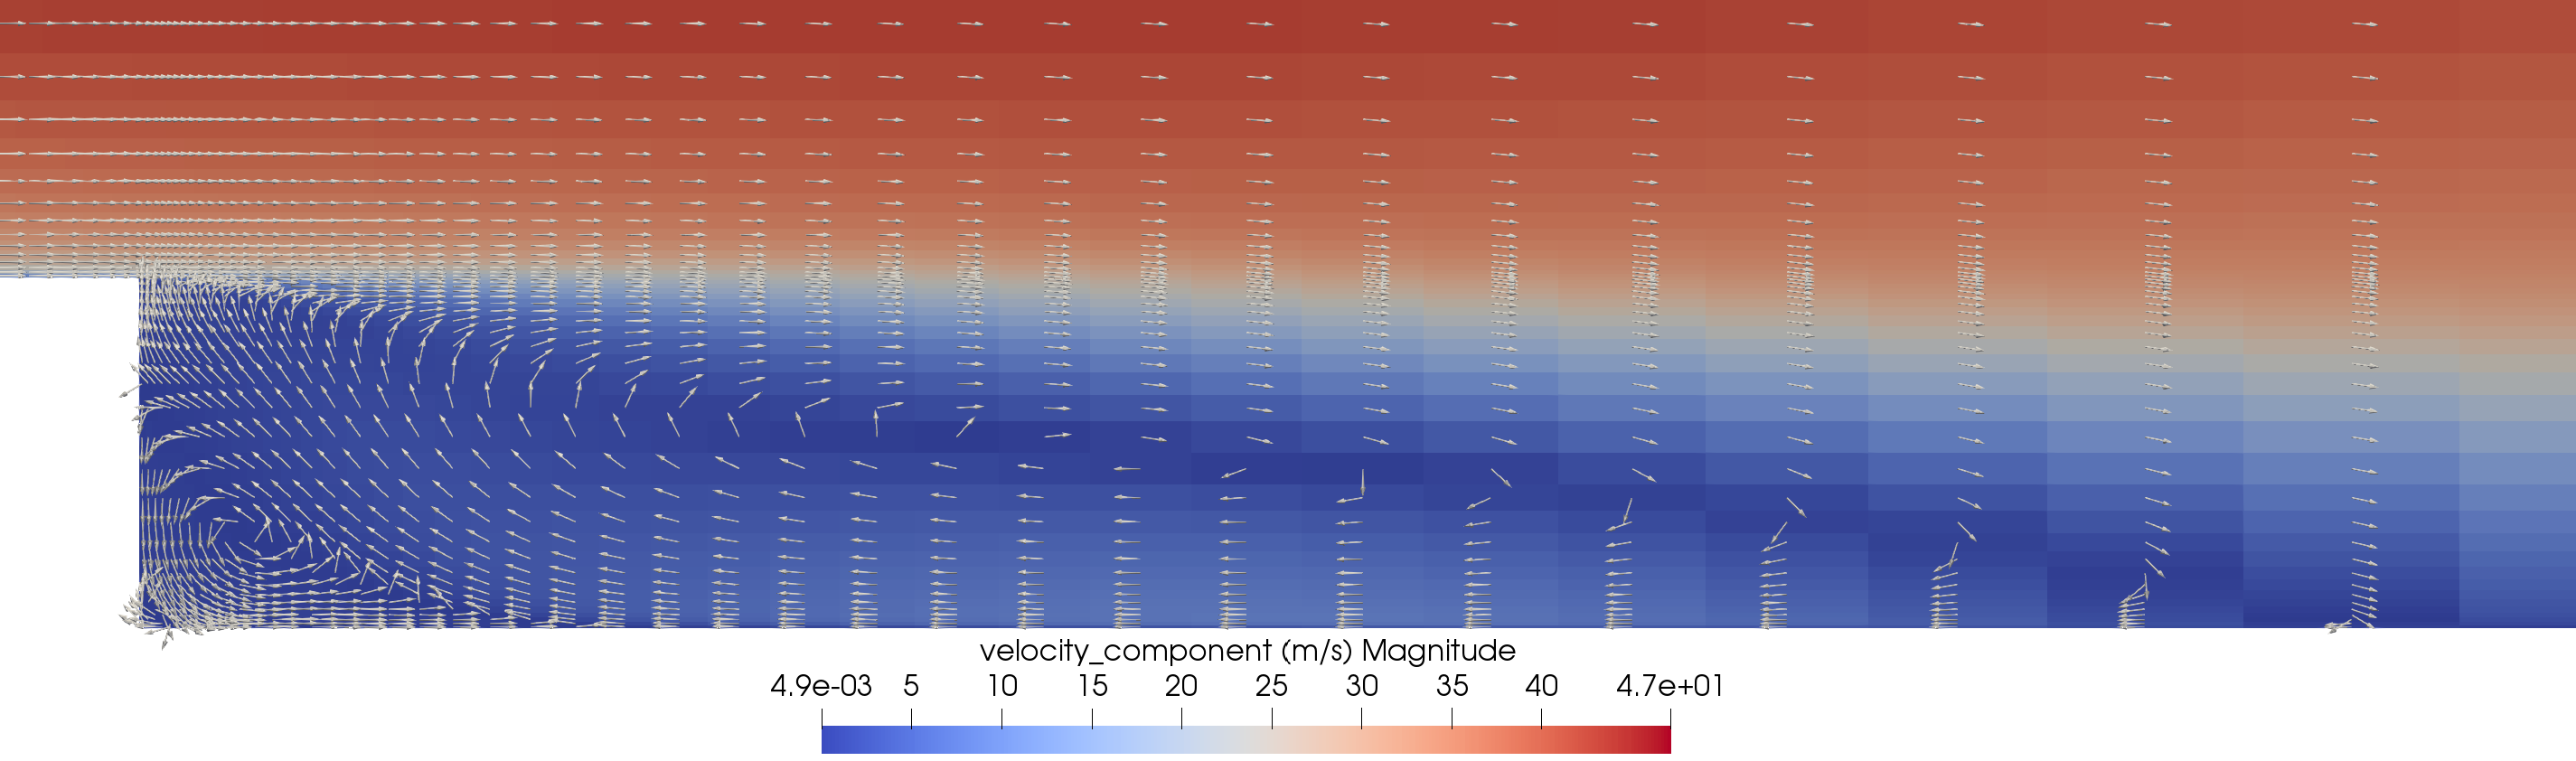
\includegraphics[width=0.9\textwidth]{bfs_glimphs.png}
	\end{figure}
\end{itemize}
\end{frame}
%%%%%%%%%%%%%%%%%%%%%%%%%%%%%%%%%%%%%%%%%%%%%%%%%%%%%%%%%%%%%%%%%%%%%%%%%%%
\begin{frame}{Coupled problem with shallow cavities}
\begin{figure}
	\centering
	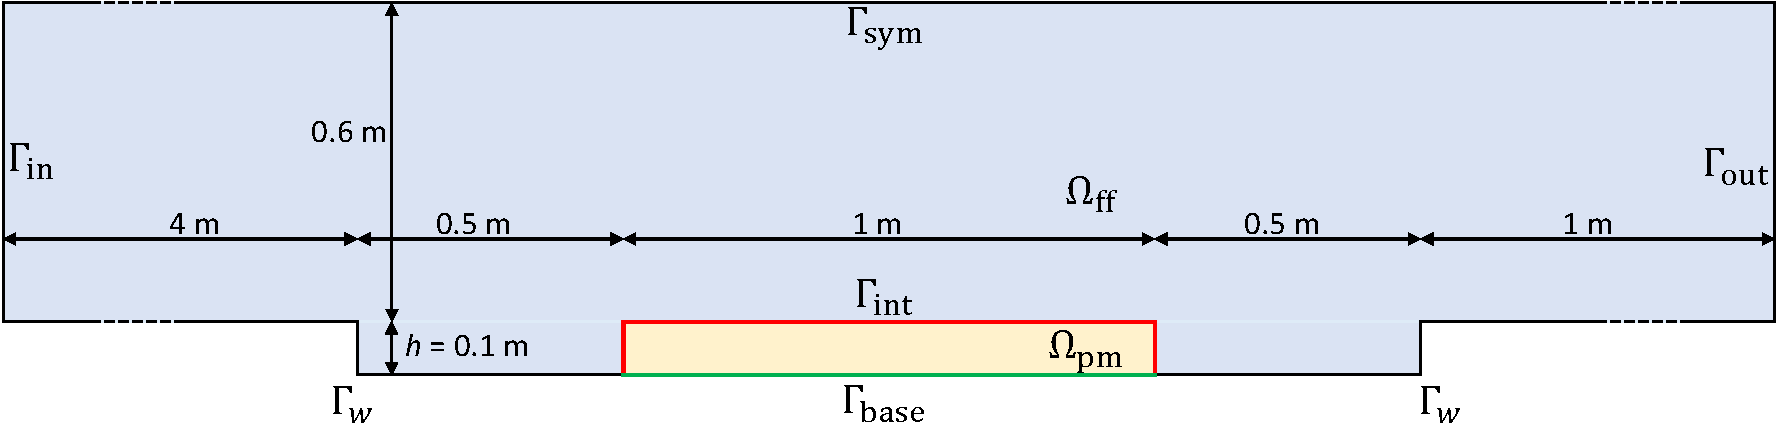
\includegraphics[width=\textwidth]{cavities_multidomain_slides.pdf}
\end{figure}
Flow in a channel with two shallow cavities on the lower boundary and a porous-medium 
between them.
\begin{itemize}
	\item $Re=60000$.
	\item Permeability ranging from $\SI{3.1e-12}{m^2}$ to $\SI{3.1e-6}{m^2}$.
	\item $\alpha_\text{BJ} = 2$, $C_F=0.55$.
\end{itemize}
\end{frame}
%%%%%%%%%%%%%%%%%%%%%%%%%%%%%%%%%%%%%%%%%%%%%%%%%%%%%%%%%%%%%%%%%%%%%%%%
\begin{frame}{Coupled problem with shallow cavities}
\begin{figure}
	\centering
	\hspace{-0.5cm}
	% This file was created by matlab2tikz.
%
\definecolor{mycolor1}{rgb}{0.00000,0.44700,0.74100}%
\definecolor{mycolor2}{rgb}{0.85000,0.32500,0.09800}%
\definecolor{mycolor3}{rgb}{0.92900,0.69400,0.12500}%
\definecolor{mycolor4}{rgb}{0.49400,0.18400,0.55600}%
\definecolor{mycolor5}{rgb}{0.46600,0.67400,0.18800}%
\definecolor{mycolor6}{rgb}{0.30100,0.74500,0.93300}%
\definecolor{mycolor7}{rgb}{0.63500,0.07800,0.18400}%
%
\begin{tikzpicture}

\begin{axis}[%
width=0.951\bfswidth,
height=0.75\roughheight,
at={(0\bfswidth,0\roughheight)},
scale only axis,
xmin=3.5,
xmax=7,
xlabel={$x$ [m]},
ymin=0,
ymax=0.45,
ylabel={$u$ [m/s]},
axis background/.style={fill=white},
xmajorgrids,
ymajorgrids,
legend style={at={(0.01,0.02)}, anchor=south west, legend cell align=left, align=left, font=\tiny}
]
\addplot [color=mycolor7, line width=1.0pt]
  table[row sep=crcr]{%
3.505	0.262726\\
3.51	0.262682\\
3.515	0.262682\\
3.52	0.262682\\
3.525	0.262682\\
3.53	0.262682\\
3.535	0.262682\\
3.54	0.262682\\
3.545	0.262682\\
3.55	0.262682\\
3.555	0.262682\\
3.56	0.262644\\
3.565	0.262644\\
3.57	0.262644\\
3.575	0.262644\\
3.58	0.262644\\
3.585	0.262644\\
3.59	0.262644\\
3.595	0.262644\\
3.6	0.262644\\
3.605	0.262611\\
3.61	0.262611\\
3.615	0.262611\\
3.62	0.262611\\
3.625	0.262611\\
3.63	0.262611\\
3.635	0.262611\\
3.64	0.262611\\
3.645	0.262584\\
3.65	0.262584\\
3.655	0.262584\\
3.66	0.262584\\
3.665	0.262584\\
3.67	0.262584\\
3.675	0.262584\\
3.68	0.262584\\
3.685	0.262563\\
3.69	0.262563\\
3.695	0.262563\\
3.7	0.262563\\
3.705	0.262563\\
3.71	0.262563\\
3.715	0.262563\\
3.72	0.262548\\
3.725	0.262548\\
3.73	0.262548\\
3.735	0.262548\\
3.74	0.262548\\
3.745	0.262548\\
3.75	0.26254\\
3.755	0.26254\\
3.76	0.26254\\
3.765	0.26254\\
3.77	0.26254\\
3.775	0.262539\\
3.78	0.262539\\
3.785	0.262539\\
3.79	0.262539\\
3.795	0.262539\\
3.8	0.262539\\
3.805	0.262545\\
3.81	0.262545\\
3.815	0.262545\\
3.82	0.262545\\
3.825	0.262557\\
3.83	0.262557\\
3.835	0.262557\\
3.84	0.262557\\
3.845	0.262578\\
3.85	0.262578\\
3.855	0.262578\\
3.86	0.262578\\
3.865	0.262608\\
3.87	0.262608\\
3.875	0.262608\\
3.88	0.262608\\
3.885	0.26265\\
3.89	0.26265\\
3.895	0.26265\\
3.9	0.262705\\
3.905	0.262705\\
3.91	0.262705\\
3.915	0.262775\\
3.92	0.262775\\
3.925	0.262864\\
3.93	0.262864\\
3.935	0.262864\\
3.94	0.262976\\
3.945	0.262976\\
3.95	0.263118\\
3.955	0.263118\\
3.96	0.263299\\
3.965	0.263299\\
3.97	0.263536\\
3.975	0.263855\\
3.98	0.263855\\
3.985	0.264312\\
3.99	0.265041\\
3.995	0.266674\\
4	0.270485\\
4.005	0.270485\\
4.01	0.276267\\
4.015	0.282429\\
4.02	0.28822\\
4.025	0.293482\\
4.03	0.298192\\
4.035	0.30243\\
4.04	0.30627\\
4.045	0.309769\\
4.05	0.31298\\
4.055	0.315951\\
4.06	0.318708\\
4.065	0.321269\\
4.07	0.323655\\
4.075	0.325893\\
4.08	0.328008\\
4.085	0.330021\\
4.09	0.331957\\
4.095	0.333836\\
4.1	0.335681\\
4.105	0.337509\\
4.11	0.339329\\
4.115	0.34115\\
4.12	0.342984\\
4.125	0.344835\\
4.13	0.346708\\
4.135	0.348606\\
4.14	0.350533\\
4.145	0.352485\\
4.15	0.354458\\
4.155	0.356445\\
4.16	0.358439\\
4.165	0.360433\\
4.17	0.362417\\
4.175	0.364386\\
4.18	0.366334\\
4.185	0.368252\\
4.19	0.370133\\
4.195	0.371973\\
4.2	0.373768\\
4.205	0.375515\\
4.21	0.377211\\
4.215	0.378852\\
4.22	0.380437\\
4.225	0.381964\\
4.23	0.383432\\
4.235	0.38484\\
4.24	0.386188\\
4.245	0.387474\\
4.25	0.388699\\
4.255	0.389864\\
4.26	0.390969\\
4.265	0.392014\\
4.27	0.393001\\
4.275	0.393932\\
4.28	0.394809\\
4.285	0.395633\\
4.29	0.396406\\
4.295	0.397132\\
4.3	0.397814\\
4.305	0.398455\\
4.31	0.399058\\
4.315	0.399629\\
4.32	0.400172\\
4.325	0.400691\\
4.33	0.401192\\
4.335	0.401679\\
4.34	0.402158\\
4.345	0.402631\\
4.35	0.403103\\
4.355	0.403576\\
4.36	0.404054\\
4.365	0.404538\\
4.37	0.405029\\
4.375	0.405527\\
4.38	0.406029\\
4.385	0.406529\\
4.39	0.407016\\
4.395	0.40748\\
4.4	0.407905\\
4.405	0.408275\\
4.41	0.408563\\
4.415	0.408727\\
4.42	0.408717\\
4.425	0.408478\\
4.43	0.407938\\
4.435	0.407011\\
4.44	0.405602\\
4.445	0.40361\\
4.45	0.400924\\
4.455	0.397429\\
4.46	0.39301\\
4.465	0.387553\\
4.47	0.380921\\
4.475	0.372881\\
4.48	0.362988\\
4.485	0.350659\\
4.49	0.334877\\
4.495	0.312452\\
4.5	0.277513\\
4.505	0.247668\\
4.51	0.220566\\
4.515	0.181727\\
4.52	0.144337\\
4.525	0.114793\\
4.53	0.0942918\\
4.535	0.0804939\\
4.54	0.0708964\\
4.545	0.0638136\\
4.55	0.0638136\\
4.555	0.0582299\\
4.56	0.0535857\\
4.565	0.0496154\\
4.57	0.0496154\\
4.575	0.0461737\\
4.58	0.0431666\\
4.585	0.0405245\\
4.59	0.0405245\\
4.595	0.0381943\\
4.6	0.0361348\\
4.605	0.0361348\\
4.61	0.0343122\\
4.615	0.0326982\\
4.62	0.0326982\\
4.625	0.0312711\\
4.63	0.0312711\\
4.635	0.030016\\
4.64	0.0289246\\
4.645	0.0289246\\
4.65	0.0279936\\
4.655	0.0279936\\
4.66	0.0272273\\
4.665	0.0272273\\
4.67	0.0266245\\
4.675	0.0266245\\
4.68	0.0261872\\
4.685	0.0259703\\
4.69	0.0259703\\
4.695	0.0259813\\
4.7	0.0259813\\
4.705	0.0262056\\
4.71	0.0262056\\
4.715	0.0267041\\
4.72	0.0267041\\
4.725	0.0267041\\
4.73	0.0275181\\
4.735	0.0275181\\
4.74	0.0286666\\
4.745	0.0286666\\
4.75	0.0301918\\
4.755	0.0301918\\
4.76	0.0321096\\
4.765	0.0321096\\
4.77	0.0344644\\
4.775	0.0344644\\
4.78	0.0344644\\
4.785	0.0373251\\
4.79	0.0373251\\
4.795	0.0407252\\
4.8	0.0407252\\
4.805	0.0407252\\
4.81	0.0446996\\
4.815	0.0446996\\
4.82	0.0492876\\
4.825	0.0492876\\
4.83	0.0492876\\
4.835	0.0545462\\
4.84	0.0545462\\
4.845	0.0545462\\
4.85	0.0605654\\
4.855	0.0605654\\
4.86	0.0674542\\
4.865	0.0674542\\
4.87	0.0674542\\
4.875	0.0753167\\
4.88	0.0753167\\
4.885	0.0753167\\
4.89	0.0842586\\
4.895	0.0842586\\
4.9	0.0842586\\
4.905	0.0944167\\
4.91	0.0944167\\
4.915	0.0944167\\
4.92	0.105935\\
4.925	0.105935\\
4.93	0.105935\\
4.935	0.118823\\
4.94	0.118823\\
4.945	0.118823\\
4.95	0.13289\\
4.955	0.13289\\
4.96	0.13289\\
4.965	0.13289\\
4.97	0.147714\\
4.975	0.147714\\
4.98	0.147714\\
4.985	0.162675\\
4.99	0.162675\\
4.995	0.162675\\
5	0.162675\\
5.005	0.177097\\
5.01	0.177097\\
5.015	0.177097\\
5.02	0.190503\\
5.025	0.190503\\
5.03	0.190503\\
5.035	0.202627\\
5.04	0.202627\\
5.045	0.202627\\
5.05	0.202627\\
5.055	0.213247\\
5.06	0.213247\\
5.065	0.213247\\
5.07	0.22241\\
5.075	0.22241\\
5.08	0.22241\\
5.085	0.230383\\
5.09	0.230383\\
5.095	0.230383\\
5.1	0.237383\\
5.105	0.237383\\
5.11	0.237383\\
5.115	0.243574\\
5.12	0.243574\\
5.125	0.243574\\
5.13	0.249073\\
5.135	0.249073\\
5.14	0.249073\\
5.145	0.253971\\
5.15	0.253971\\
5.155	0.258338\\
5.16	0.258338\\
5.165	0.258338\\
5.17	0.262239\\
5.175	0.262239\\
5.18	0.262239\\
5.185	0.265723\\
5.19	0.265723\\
5.195	0.268837\\
5.2	0.268837\\
5.205	0.268837\\
5.21	0.271621\\
5.215	0.271621\\
5.22	0.274108\\
5.225	0.274108\\
5.23	0.274108\\
5.235	0.276331\\
5.24	0.276331\\
5.245	0.278316\\
5.25	0.278316\\
5.255	0.280089\\
5.26	0.280089\\
5.265	0.28167\\
5.27	0.28167\\
5.275	0.28308\\
5.28	0.28308\\
5.285	0.28308\\
5.29	0.284336\\
5.295	0.284336\\
5.3	0.285453\\
5.305	0.285453\\
5.31	0.286445\\
5.315	0.286445\\
5.32	0.287325\\
5.325	0.288104\\
5.33	0.288104\\
5.335	0.288793\\
5.34	0.288793\\
5.345	0.2894\\
5.35	0.2894\\
5.355	0.289933\\
5.36	0.289933\\
5.365	0.2904\\
5.37	0.290809\\
5.375	0.290809\\
5.38	0.291164\\
5.385	0.291164\\
5.39	0.291471\\
5.395	0.291735\\
5.4	0.291735\\
5.405	0.291962\\
5.41	0.292154\\
5.415	0.292154\\
5.42	0.292315\\
5.425	0.292449\\
5.43	0.292559\\
5.435	0.292559\\
5.44	0.292647\\
5.445	0.292716\\
5.45	0.292767\\
5.455	0.292767\\
5.46	0.292804\\
5.465	0.292828\\
5.47	0.292843\\
5.475	0.292853\\
5.48	0.292869\\
5.485	0.292915\\
5.49	0.293109\\
5.495	0.294023\\
5.5	0.296593\\
5.505	0.296593\\
5.51	0.300504\\
5.515	0.304594\\
5.52	0.308373\\
5.525	0.311702\\
5.53	0.314576\\
5.535	0.317014\\
5.54	0.319061\\
5.545	0.320796\\
5.55	0.322305\\
5.555	0.323654\\
5.56	0.324878\\
5.565	0.325998\\
5.57	0.327036\\
5.575	0.328014\\
5.58	0.328954\\
5.585	0.329871\\
5.59	0.330778\\
5.595	0.331682\\
5.6	0.332593\\
5.605	0.333517\\
5.61	0.334462\\
5.615	0.335437\\
5.62	0.336451\\
5.625	0.337505\\
5.63	0.338598\\
5.635	0.339729\\
5.64	0.340898\\
5.645	0.342105\\
5.65	0.343349\\
5.655	0.344626\\
5.66	0.345933\\
5.665	0.347267\\
5.67	0.348623\\
5.675	0.349999\\
5.68	0.35139\\
5.685	0.352788\\
5.69	0.354187\\
5.695	0.355578\\
5.7	0.356954\\
5.705	0.358307\\
5.71	0.359631\\
5.715	0.360919\\
5.72	0.362166\\
5.725	0.363368\\
5.73	0.364521\\
5.735	0.365621\\
5.74	0.366668\\
5.745	0.367658\\
5.75	0.368594\\
5.755	0.369473\\
5.76	0.370295\\
5.765	0.37106\\
5.77	0.371768\\
5.775	0.372419\\
5.78	0.373014\\
5.785	0.373554\\
5.79	0.374039\\
5.795	0.374471\\
5.8	0.374851\\
5.805	0.375182\\
5.81	0.375465\\
5.815	0.375703\\
5.82	0.3759\\
5.825	0.37606\\
5.83	0.376184\\
5.835	0.376276\\
5.84	0.376338\\
5.845	0.376375\\
5.85	0.376386\\
5.855	0.376375\\
5.86	0.376342\\
5.865	0.376283\\
5.87	0.376197\\
5.875	0.37608\\
5.88	0.375925\\
5.885	0.375724\\
5.89	0.375463\\
5.895	0.375127\\
5.9	0.374699\\
5.905	0.374156\\
5.91	0.373471\\
5.915	0.372611\\
5.92	0.371537\\
5.925	0.370203\\
5.93	0.368564\\
5.935	0.366568\\
5.94	0.364163\\
5.945	0.361295\\
5.95	0.357892\\
5.955	0.353866\\
5.96	0.349093\\
5.965	0.343406\\
5.97	0.336586\\
5.975	0.328335\\
5.98	0.31829\\
5.985	0.30607\\
5.99	0.291239\\
5.995	0.275687\\
6	0.28812\\
6.005	0.191094\\
6.01	0.191094\\
6.015	0.165779\\
6.02	0.162093\\
6.025	0.168067\\
6.03	0.168067\\
6.035	0.177057\\
6.04	0.186755\\
6.045	0.186755\\
6.05	0.196155\\
6.055	0.196155\\
6.06	0.204619\\
6.065	0.204619\\
6.07	0.212242\\
6.075	0.212242\\
6.08	0.219043\\
6.085	0.219043\\
6.09	0.219043\\
6.095	0.225134\\
6.1	0.225134\\
6.105	0.225134\\
6.11	0.230569\\
6.115	0.230569\\
6.12	0.230569\\
6.125	0.235415\\
6.13	0.235415\\
6.135	0.235415\\
6.14	0.23969\\
6.145	0.23969\\
6.15	0.23969\\
6.155	0.23969\\
6.16	0.243427\\
6.165	0.243427\\
6.17	0.243427\\
6.175	0.243427\\
6.18	0.246671\\
6.185	0.246671\\
6.19	0.246671\\
6.195	0.246671\\
6.2	0.246671\\
6.205	0.249427\\
6.21	0.249427\\
6.215	0.249427\\
6.22	0.249427\\
6.225	0.249427\\
6.23	0.251725\\
6.235	0.251725\\
6.24	0.251725\\
6.245	0.251725\\
6.25	0.251725\\
6.255	0.253618\\
6.26	0.253618\\
6.265	0.253618\\
6.27	0.253618\\
6.275	0.253618\\
6.28	0.253618\\
6.285	0.255137\\
6.29	0.255137\\
6.295	0.255137\\
6.3	0.255137\\
6.305	0.255137\\
6.31	0.255137\\
6.315	0.255137\\
6.32	0.256311\\
6.325	0.256311\\
6.33	0.256311\\
6.335	0.256311\\
6.34	0.256311\\
6.345	0.256311\\
6.35	0.256311\\
6.355	0.256311\\
6.36	0.257182\\
6.365	0.257182\\
6.37	0.257182\\
6.375	0.257182\\
6.38	0.257182\\
6.385	0.257182\\
6.39	0.257182\\
6.395	0.257182\\
6.4	0.257808\\
6.405	0.257808\\
6.41	0.257808\\
6.415	0.257808\\
6.42	0.257808\\
6.425	0.257808\\
6.43	0.257808\\
6.435	0.257808\\
6.44	0.257808\\
6.445	0.258229\\
6.45	0.258229\\
6.455	0.258229\\
6.46	0.258229\\
6.465	0.258229\\
6.47	0.258229\\
6.475	0.258229\\
6.48	0.258229\\
6.485	0.258229\\
6.49	0.258486\\
6.495	0.258486\\
6.5	0.258486\\
6.505	0.258486\\
6.51	0.258486\\
6.515	0.258486\\
6.52	0.258486\\
6.525	0.258486\\
6.53	0.258486\\
6.535	0.258486\\
6.54	0.258486\\
6.545	0.258604\\
6.55	0.258604\\
6.555	0.258604\\
6.56	0.258604\\
6.565	0.258604\\
6.57	0.258604\\
6.575	0.258604\\
6.58	0.258604\\
6.585	0.258604\\
6.59	0.258604\\
6.595	0.258604\\
6.6	0.258604\\
6.605	0.258618\\
6.61	0.258618\\
6.615	0.258618\\
6.62	0.258618\\
6.625	0.258618\\
6.63	0.258618\\
6.635	0.258618\\
6.64	0.258618\\
6.645	0.258618\\
6.65	0.258618\\
6.655	0.258618\\
6.66	0.258618\\
6.665	0.258618\\
6.67	0.258575\\
6.675	0.258575\\
6.68	0.258575\\
6.685	0.258575\\
6.69	0.258575\\
6.695	0.258575\\
6.7	0.258575\\
6.705	0.258575\\
6.71	0.258575\\
6.715	0.258575\\
6.72	0.258575\\
6.725	0.258575\\
6.73	0.258575\\
6.735	0.258575\\
6.74	0.258482\\
6.745	0.258482\\
6.75	0.258482\\
6.755	0.258482\\
6.76	0.258482\\
6.765	0.258482\\
6.77	0.258482\\
6.775	0.258482\\
6.78	0.258482\\
6.785	0.258482\\
6.79	0.258482\\
6.795	0.258482\\
6.8	0.258482\\
6.805	0.258482\\
6.81	0.258482\\
6.815	0.258482\\
6.82	0.25848\\
6.825	0.25848\\
6.83	0.25848\\
6.835	0.25848\\
6.84	0.25848\\
6.845	0.25848\\
6.85	0.25848\\
6.855	0.25848\\
6.86	0.25848\\
6.865	0.25848\\
6.87	0.25848\\
6.875	0.25848\\
6.88	0.25848\\
6.885	0.25848\\
6.89	0.25848\\
6.895	0.25848\\
6.9	0.25848\\
6.905	0.258518\\
6.91	0.258518\\
6.915	0.258518\\
6.92	0.258518\\
6.925	0.258518\\
6.93	0.258518\\
6.935	0.258518\\
6.94	0.258518\\
6.945	0.258518\\
6.95	0.258518\\
6.955	0.258518\\
6.96	0.258518\\
6.965	0.258518\\
6.97	0.258518\\
6.975	0.258518\\
6.98	0.258518\\
6.985	0.258518\\
6.99	0.258518\\
6.995	0.258518\\
7	0.258518\\
};
\addlegendentry{$\mathrm{K}$ = 3.1e-6 $\si{m^2}$}

\addplot [color=mycolor6, line width=1.0pt]
  table[row sep=crcr]{%
3.505	0.26269\\
3.51	0.262634\\
3.515	0.262634\\
3.52	0.262634\\
3.525	0.262634\\
3.53	0.262634\\
3.535	0.262634\\
3.54	0.262634\\
3.545	0.262634\\
3.55	0.262634\\
3.555	0.262634\\
3.56	0.262582\\
3.565	0.262582\\
3.57	0.262582\\
3.575	0.262582\\
3.58	0.262582\\
3.585	0.262582\\
3.59	0.262582\\
3.595	0.262582\\
3.6	0.262582\\
3.605	0.262533\\
3.61	0.262533\\
3.615	0.262533\\
3.62	0.262533\\
3.625	0.262533\\
3.63	0.262533\\
3.635	0.262533\\
3.64	0.262533\\
3.645	0.262487\\
3.65	0.262487\\
3.655	0.262487\\
3.66	0.262487\\
3.665	0.262487\\
3.67	0.262487\\
3.675	0.262487\\
3.68	0.262487\\
3.685	0.262445\\
3.69	0.262445\\
3.695	0.262445\\
3.7	0.262445\\
3.705	0.262445\\
3.71	0.262445\\
3.715	0.262445\\
3.72	0.262407\\
3.725	0.262407\\
3.73	0.262407\\
3.735	0.262407\\
3.74	0.262407\\
3.745	0.262407\\
3.75	0.262372\\
3.755	0.262372\\
3.76	0.262372\\
3.765	0.262372\\
3.77	0.262372\\
3.775	0.262343\\
3.78	0.262343\\
3.785	0.262343\\
3.79	0.262343\\
3.795	0.262343\\
3.8	0.262343\\
3.805	0.262318\\
3.81	0.262318\\
3.815	0.262318\\
3.82	0.262318\\
3.825	0.2623\\
3.83	0.2623\\
3.835	0.2623\\
3.84	0.2623\\
3.845	0.262288\\
3.85	0.262288\\
3.855	0.262288\\
3.86	0.262288\\
3.865	0.262284\\
3.87	0.262284\\
3.875	0.262284\\
3.88	0.262284\\
3.885	0.26229\\
3.89	0.26229\\
3.895	0.26229\\
3.9	0.262305\\
3.905	0.262305\\
3.91	0.262305\\
3.915	0.26233\\
3.92	0.26233\\
3.925	0.262372\\
3.93	0.262372\\
3.935	0.262372\\
3.94	0.262433\\
3.945	0.262433\\
3.95	0.262519\\
3.955	0.262519\\
3.96	0.262641\\
3.965	0.262641\\
3.97	0.262812\\
3.975	0.263058\\
3.98	0.263058\\
3.985	0.263433\\
3.99	0.264068\\
3.995	0.265556\\
4	0.269173\\
4.005	0.269173\\
4.01	0.274767\\
4.015	0.28074\\
4.02	0.286326\\
4.025	0.291386\\
4.03	0.295908\\
4.035	0.299969\\
4.04	0.303649\\
4.045	0.307005\\
4.05	0.310083\\
4.055	0.312921\\
4.06	0.315544\\
4.065	0.31797\\
4.07	0.320224\\
4.075	0.322334\\
4.08	0.324325\\
4.085	0.326218\\
4.09	0.328037\\
4.095	0.329804\\
4.1	0.33154\\
4.105	0.333259\\
4.11	0.334971\\
4.115	0.336686\\
4.12	0.338414\\
4.125	0.34016\\
4.13	0.341929\\
4.135	0.343725\\
4.14	0.345549\\
4.145	0.347398\\
4.15	0.349268\\
4.155	0.351151\\
4.16	0.353039\\
4.165	0.354924\\
4.17	0.356799\\
4.175	0.358655\\
4.18	0.360484\\
4.185	0.362281\\
4.19	0.36404\\
4.195	0.365756\\
4.2	0.367424\\
4.205	0.36904\\
4.21	0.3706\\
4.215	0.372102\\
4.22	0.373543\\
4.225	0.374921\\
4.23	0.376235\\
4.235	0.377484\\
4.24	0.378667\\
4.245	0.379783\\
4.25	0.380833\\
4.255	0.381816\\
4.26	0.382734\\
4.265	0.383588\\
4.27	0.384378\\
4.275	0.385107\\
4.28	0.385775\\
4.285	0.386386\\
4.29	0.38694\\
4.295	0.38744\\
4.3	0.387891\\
4.305	0.388294\\
4.31	0.388655\\
4.315	0.388976\\
4.32	0.389262\\
4.325	0.389519\\
4.33	0.38975\\
4.335	0.389961\\
4.34	0.390156\\
4.345	0.390337\\
4.35	0.390509\\
4.355	0.390674\\
4.36	0.390835\\
4.365	0.390993\\
4.37	0.391149\\
4.375	0.391299\\
4.38	0.39144\\
4.385	0.391564\\
4.39	0.391662\\
4.395	0.39172\\
4.4	0.391723\\
4.405	0.391651\\
4.41	0.391471\\
4.415	0.391136\\
4.42	0.390593\\
4.425	0.389779\\
4.43	0.388624\\
4.435	0.387048\\
4.44	0.384962\\
4.445	0.382276\\
4.45	0.378902\\
4.455	0.374757\\
4.46	0.369764\\
4.465	0.363783\\
4.47	0.356596\\
4.475	0.347891\\
4.48	0.337221\\
4.485	0.324005\\
4.49	0.307261\\
4.495	0.284512\\
4.5	0.260133\\
4.505	0.229546\\
4.51	0.186773\\
4.515	0.143929\\
4.52	0.111636\\
4.525	0.0911823\\
4.53	0.0784582\\
4.535	0.0701259\\
4.54	0.0642528\\
4.545	0.0598307\\
4.55	0.0598307\\
4.555	0.0563841\\
4.56	0.0536946\\
4.565	0.0516593\\
4.57	0.0516593\\
4.575	0.0502206\\
4.58	0.0494158\\
4.585	0.0491474\\
4.59	0.0491474\\
4.595	0.049469\\
4.6	0.0506071\\
4.605	0.0506071\\
4.61	0.0525077\\
4.615	0.0552416\\
4.62	0.0552416\\
4.625	0.0589932\\
4.63	0.0589932\\
4.635	0.0638691\\
4.64	0.0700044\\
4.645	0.0700044\\
4.65	0.0775865\\
4.655	0.0775865\\
4.66	0.0868303\\
4.665	0.0868303\\
4.67	0.0978423\\
4.675	0.0978423\\
4.68	0.110489\\
4.685	0.124266\\
4.69	0.124266\\
4.695	0.138428\\
4.7	0.138428\\
4.705	0.152347\\
4.71	0.152347\\
4.715	0.165642\\
4.72	0.165642\\
4.725	0.165642\\
4.73	0.178107\\
4.735	0.178107\\
4.74	0.189543\\
4.745	0.189543\\
4.75	0.199767\\
4.755	0.199767\\
4.76	0.208802\\
4.765	0.208802\\
4.77	0.216803\\
4.775	0.216803\\
4.78	0.216803\\
4.785	0.223904\\
4.79	0.223904\\
4.795	0.230212\\
4.8	0.230212\\
4.805	0.230212\\
4.81	0.235818\\
4.815	0.235818\\
4.82	0.240798\\
4.825	0.240798\\
4.83	0.240798\\
4.835	0.245215\\
4.84	0.245215\\
4.845	0.245215\\
4.85	0.249125\\
4.855	0.249125\\
4.86	0.252573\\
4.865	0.252573\\
4.87	0.252573\\
4.875	0.255604\\
4.88	0.255604\\
4.885	0.255604\\
4.89	0.258256\\
4.895	0.258256\\
4.9	0.258256\\
4.905	0.260566\\
4.91	0.260566\\
4.915	0.260566\\
4.92	0.262568\\
4.925	0.262568\\
4.93	0.262568\\
4.935	0.264296\\
4.94	0.264296\\
4.945	0.264296\\
4.95	0.265778\\
4.955	0.265778\\
4.96	0.265778\\
4.965	0.265778\\
4.97	0.267044\\
4.975	0.267044\\
4.98	0.267044\\
4.985	0.268123\\
4.99	0.268123\\
4.995	0.268123\\
5	0.268123\\
5.005	0.269025\\
5.01	0.269025\\
5.015	0.269025\\
5.02	0.269757\\
5.025	0.269757\\
5.03	0.269757\\
5.035	0.270345\\
5.04	0.270345\\
5.045	0.270345\\
5.05	0.270345\\
5.055	0.270823\\
5.06	0.270823\\
5.065	0.270823\\
5.07	0.271215\\
5.075	0.271215\\
5.08	0.271215\\
5.085	0.271538\\
5.09	0.271538\\
5.095	0.271538\\
5.1	0.271807\\
5.105	0.271807\\
5.11	0.271807\\
5.115	0.27203\\
5.12	0.27203\\
5.125	0.27203\\
5.13	0.272217\\
5.135	0.272217\\
5.14	0.272217\\
5.145	0.272373\\
5.15	0.272373\\
5.155	0.272505\\
5.16	0.272505\\
5.165	0.272505\\
5.17	0.272616\\
5.175	0.272616\\
5.18	0.272616\\
5.185	0.27271\\
5.19	0.27271\\
5.195	0.272789\\
5.2	0.272789\\
5.205	0.272789\\
5.21	0.272857\\
5.215	0.272857\\
5.22	0.272914\\
5.225	0.272914\\
5.23	0.272914\\
5.235	0.272963\\
5.24	0.272963\\
5.245	0.273004\\
5.25	0.273004\\
5.255	0.273039\\
5.26	0.273039\\
5.265	0.273069\\
5.27	0.273069\\
5.275	0.273094\\
5.28	0.273094\\
5.285	0.273094\\
5.29	0.273116\\
5.295	0.273116\\
5.3	0.273134\\
5.305	0.273134\\
5.31	0.273149\\
5.315	0.273149\\
5.32	0.273162\\
5.325	0.273173\\
5.33	0.273173\\
5.335	0.273183\\
5.34	0.273183\\
5.345	0.273192\\
5.35	0.273192\\
5.355	0.2732\\
5.36	0.2732\\
5.365	0.273208\\
5.37	0.273215\\
5.375	0.273215\\
5.38	0.273223\\
5.385	0.273223\\
5.39	0.273232\\
5.395	0.273242\\
5.4	0.273242\\
5.405	0.273253\\
5.41	0.273266\\
5.415	0.273266\\
5.42	0.273281\\
5.425	0.273298\\
5.43	0.273318\\
5.435	0.273318\\
5.44	0.273341\\
5.445	0.273369\\
5.45	0.273402\\
5.455	0.273402\\
5.46	0.273442\\
5.465	0.273491\\
5.47	0.273556\\
5.475	0.273643\\
5.48	0.273766\\
5.485	0.27396\\
5.49	0.274415\\
5.495	0.275502\\
5.5	0.278192\\
5.505	0.278192\\
5.51	0.282458\\
5.515	0.287025\\
5.52	0.29131\\
5.525	0.295177\\
5.53	0.298615\\
5.535	0.301683\\
5.54	0.304446\\
5.545	0.306953\\
5.55	0.309241\\
5.555	0.311346\\
5.56	0.313291\\
5.565	0.315099\\
5.57	0.316796\\
5.575	0.318404\\
5.58	0.319938\\
5.585	0.321412\\
5.59	0.322836\\
5.595	0.324218\\
5.6	0.325569\\
5.605	0.326904\\
5.61	0.328235\\
5.615	0.329566\\
5.62	0.330903\\
5.625	0.332253\\
5.63	0.333623\\
5.635	0.335018\\
5.64	0.336441\\
5.645	0.337895\\
5.65	0.339381\\
5.655	0.340899\\
5.66	0.342448\\
5.665	0.344021\\
5.67	0.345611\\
5.675	0.34721\\
5.68	0.348811\\
5.685	0.350404\\
5.69	0.351981\\
5.695	0.353536\\
5.7	0.35506\\
5.705	0.356548\\
5.71	0.357993\\
5.715	0.359392\\
5.72	0.36074\\
5.725	0.362036\\
5.73	0.363277\\
5.735	0.364461\\
5.74	0.365587\\
5.745	0.366652\\
5.75	0.367657\\
5.755	0.368601\\
5.76	0.369482\\
5.765	0.370302\\
5.77	0.371058\\
5.775	0.371754\\
5.78	0.372389\\
5.785	0.372964\\
5.79	0.373482\\
5.795	0.373944\\
5.8	0.374351\\
5.805	0.374707\\
5.81	0.375016\\
5.815	0.375279\\
5.82	0.3755\\
5.825	0.375683\\
5.83	0.375831\\
5.835	0.375946\\
5.84	0.376033\\
5.845	0.376093\\
5.85	0.37613\\
5.855	0.376142\\
5.86	0.376132\\
5.865	0.376101\\
5.87	0.376045\\
5.875	0.375959\\
5.88	0.375835\\
5.885	0.375667\\
5.89	0.375445\\
5.895	0.375153\\
5.9	0.374772\\
5.905	0.374276\\
5.91	0.373639\\
5.915	0.372827\\
5.92	0.371797\\
5.925	0.370504\\
5.93	0.368898\\
5.935	0.366929\\
5.94	0.36455\\
5.945	0.361706\\
5.95	0.358326\\
5.955	0.354324\\
5.96	0.349578\\
5.965	0.343924\\
5.97	0.337141\\
5.975	0.328931\\
5.98	0.318926\\
5.985	0.306745\\
5.99	0.291948\\
5.995	0.276415\\
6	0.28891\\
6.005	0.191585\\
6.01	0.191585\\
6.015	0.166242\\
6.02	0.162558\\
6.025	0.168504\\
6.03	0.168504\\
6.035	0.177446\\
6.04	0.187089\\
6.045	0.187089\\
6.05	0.196446\\
6.055	0.196446\\
6.06	0.204888\\
6.065	0.204888\\
6.07	0.212517\\
6.075	0.212517\\
6.08	0.219351\\
6.085	0.219351\\
6.09	0.219351\\
6.095	0.225486\\
6.1	0.225486\\
6.105	0.225486\\
6.11	0.230974\\
6.115	0.230974\\
6.12	0.230974\\
6.125	0.235883\\
6.13	0.235883\\
6.135	0.235883\\
6.14	0.240226\\
6.145	0.240226\\
6.15	0.240226\\
6.155	0.240226\\
6.16	0.24403\\
6.165	0.24403\\
6.17	0.24403\\
6.175	0.24403\\
6.18	0.247333\\
6.185	0.247333\\
6.19	0.247333\\
6.195	0.247333\\
6.2	0.247333\\
6.205	0.250148\\
6.21	0.250148\\
6.215	0.250148\\
6.22	0.250148\\
6.225	0.250148\\
6.23	0.252497\\
6.235	0.252497\\
6.24	0.252497\\
6.245	0.252497\\
6.25	0.252497\\
6.255	0.254422\\
6.26	0.254422\\
6.265	0.254422\\
6.27	0.254422\\
6.275	0.254422\\
6.28	0.254422\\
6.285	0.25596\\
6.29	0.25596\\
6.295	0.25596\\
6.3	0.25596\\
6.305	0.25596\\
6.31	0.25596\\
6.315	0.25596\\
6.32	0.257151\\
6.325	0.257151\\
6.33	0.257151\\
6.335	0.257151\\
6.34	0.257151\\
6.345	0.257151\\
6.35	0.257151\\
6.355	0.257151\\
6.36	0.258025\\
6.365	0.258025\\
6.37	0.258025\\
6.375	0.258025\\
6.38	0.258025\\
6.385	0.258025\\
6.39	0.258025\\
6.395	0.258025\\
6.4	0.258631\\
6.405	0.258631\\
6.41	0.258631\\
6.415	0.258631\\
6.42	0.258631\\
6.425	0.258631\\
6.43	0.258631\\
6.435	0.258631\\
6.44	0.258631\\
6.445	0.259025\\
6.45	0.259025\\
6.455	0.259025\\
6.46	0.259025\\
6.465	0.259025\\
6.47	0.259025\\
6.475	0.259025\\
6.48	0.259025\\
6.485	0.259025\\
6.49	0.259251\\
6.495	0.259251\\
6.5	0.259251\\
6.505	0.259251\\
6.51	0.259251\\
6.515	0.259251\\
6.52	0.259251\\
6.525	0.259251\\
6.53	0.259251\\
6.535	0.259251\\
6.54	0.259251\\
6.545	0.259324\\
6.55	0.259324\\
6.555	0.259324\\
6.56	0.259324\\
6.565	0.259324\\
6.57	0.259324\\
6.575	0.259324\\
6.58	0.259324\\
6.585	0.259324\\
6.59	0.259324\\
6.595	0.259324\\
6.6	0.259324\\
6.605	0.259288\\
6.61	0.259288\\
6.615	0.259288\\
6.62	0.259288\\
6.625	0.259288\\
6.63	0.259288\\
6.635	0.259288\\
6.64	0.259288\\
6.645	0.259288\\
6.65	0.259288\\
6.655	0.259288\\
6.66	0.259288\\
6.665	0.259288\\
6.67	0.259195\\
6.675	0.259195\\
6.68	0.259195\\
6.685	0.259195\\
6.69	0.259195\\
6.695	0.259195\\
6.7	0.259195\\
6.705	0.259195\\
6.71	0.259195\\
6.715	0.259195\\
6.72	0.259195\\
6.725	0.259195\\
6.73	0.259195\\
6.735	0.259195\\
6.74	0.259049\\
6.745	0.259049\\
6.75	0.259049\\
6.755	0.259049\\
6.76	0.259049\\
6.765	0.259049\\
6.77	0.259049\\
6.775	0.259049\\
6.78	0.259049\\
6.785	0.259049\\
6.79	0.259049\\
6.795	0.259049\\
6.8	0.259049\\
6.805	0.259049\\
6.81	0.259049\\
6.815	0.259049\\
6.82	0.258996\\
6.825	0.258996\\
6.83	0.258996\\
6.835	0.258996\\
6.84	0.258996\\
6.845	0.258996\\
6.85	0.258996\\
6.855	0.258996\\
6.86	0.258996\\
6.865	0.258996\\
6.87	0.258996\\
6.875	0.258996\\
6.88	0.258996\\
6.885	0.258996\\
6.89	0.258996\\
6.895	0.258996\\
6.9	0.258996\\
6.905	0.258999\\
6.91	0.258999\\
6.915	0.258999\\
6.92	0.258999\\
6.925	0.258999\\
6.93	0.258999\\
6.935	0.258999\\
6.94	0.258999\\
6.945	0.258999\\
6.95	0.258999\\
6.955	0.258999\\
6.96	0.258999\\
6.965	0.258999\\
6.97	0.258999\\
6.975	0.258999\\
6.98	0.258999\\
6.985	0.258999\\
6.99	0.258999\\
6.995	0.258999\\
7	0.258999\\
};
\addlegendentry{$\mathrm{K}$ = 3.1e-7 $\si{m^2}$}

\addplot [color=mycolor5, line width=1.0pt]
  table[row sep=crcr]{%
3.505	0.262686\\
3.51	0.26263\\
3.515	0.26263\\
3.52	0.26263\\
3.525	0.26263\\
3.53	0.26263\\
3.535	0.26263\\
3.54	0.26263\\
3.545	0.26263\\
3.55	0.26263\\
3.555	0.26263\\
3.56	0.262576\\
3.565	0.262576\\
3.57	0.262576\\
3.575	0.262576\\
3.58	0.262576\\
3.585	0.262576\\
3.59	0.262576\\
3.595	0.262576\\
3.6	0.262576\\
3.605	0.262526\\
3.61	0.262526\\
3.615	0.262526\\
3.62	0.262526\\
3.625	0.262526\\
3.63	0.262526\\
3.635	0.262526\\
3.64	0.262526\\
3.645	0.262479\\
3.65	0.262479\\
3.655	0.262479\\
3.66	0.262479\\
3.665	0.262479\\
3.67	0.262479\\
3.675	0.262479\\
3.68	0.262479\\
3.685	0.262435\\
3.69	0.262435\\
3.695	0.262435\\
3.7	0.262435\\
3.705	0.262435\\
3.71	0.262435\\
3.715	0.262435\\
3.72	0.262394\\
3.725	0.262394\\
3.73	0.262394\\
3.735	0.262394\\
3.74	0.262394\\
3.745	0.262394\\
3.75	0.262357\\
3.755	0.262357\\
3.76	0.262357\\
3.765	0.262357\\
3.77	0.262357\\
3.775	0.262324\\
3.78	0.262324\\
3.785	0.262324\\
3.79	0.262324\\
3.795	0.262324\\
3.8	0.262324\\
3.805	0.262297\\
3.81	0.262297\\
3.815	0.262297\\
3.82	0.262297\\
3.825	0.262275\\
3.83	0.262275\\
3.835	0.262275\\
3.84	0.262275\\
3.845	0.262259\\
3.85	0.262259\\
3.855	0.262259\\
3.86	0.262259\\
3.865	0.262251\\
3.87	0.262251\\
3.875	0.262251\\
3.88	0.262251\\
3.885	0.262253\\
3.89	0.262253\\
3.895	0.262253\\
3.9	0.262263\\
3.905	0.262263\\
3.91	0.262263\\
3.915	0.262285\\
3.92	0.262285\\
3.925	0.262321\\
3.93	0.262321\\
3.935	0.262321\\
3.94	0.262377\\
3.945	0.262377\\
3.95	0.262457\\
3.955	0.262457\\
3.96	0.262572\\
3.965	0.262572\\
3.97	0.262735\\
3.975	0.262974\\
3.98	0.262974\\
3.985	0.263339\\
3.99	0.263963\\
3.995	0.265435\\
4	0.26903\\
4.005	0.26903\\
4.01	0.274603\\
4.015	0.280555\\
4.02	0.286119\\
4.025	0.291156\\
4.03	0.295656\\
4.035	0.299697\\
4.04	0.303358\\
4.045	0.306697\\
4.05	0.30976\\
4.055	0.312582\\
4.06	0.315189\\
4.065	0.317599\\
4.07	0.319837\\
4.075	0.321932\\
4.08	0.323907\\
4.085	0.325786\\
4.09	0.327591\\
4.095	0.329344\\
4.1	0.331067\\
4.105	0.332773\\
4.11	0.334472\\
4.115	0.336175\\
4.12	0.33789\\
4.125	0.339623\\
4.13	0.341379\\
4.135	0.343163\\
4.14	0.344974\\
4.145	0.34681\\
4.15	0.348666\\
4.155	0.350535\\
4.16	0.352408\\
4.165	0.354279\\
4.17	0.356138\\
4.175	0.357978\\
4.18	0.35979\\
4.185	0.361569\\
4.19	0.36331\\
4.195	0.365007\\
4.2	0.366655\\
4.205	0.36825\\
4.21	0.36979\\
4.215	0.37127\\
4.22	0.372688\\
4.225	0.374043\\
4.23	0.375332\\
4.235	0.376556\\
4.24	0.377712\\
4.245	0.378801\\
4.25	0.379822\\
4.255	0.380777\\
4.26	0.381664\\
4.265	0.382486\\
4.27	0.383244\\
4.275	0.38394\\
4.28	0.384574\\
4.285	0.385149\\
4.29	0.385666\\
4.295	0.386129\\
4.3	0.386541\\
4.305	0.386904\\
4.31	0.387222\\
4.315	0.3875\\
4.32	0.38774\\
4.325	0.387949\\
4.33	0.388131\\
4.335	0.38829\\
4.34	0.388429\\
4.345	0.388553\\
4.35	0.388663\\
4.355	0.388763\\
4.36	0.388855\\
4.365	0.38894\\
4.37	0.389018\\
4.375	0.389085\\
4.38	0.389136\\
4.385	0.389164\\
4.39	0.389158\\
4.395	0.389108\\
4.4	0.388995\\
4.405	0.388796\\
4.41	0.388481\\
4.415	0.388005\\
4.42	0.387317\\
4.425	0.386356\\
4.43	0.385054\\
4.435	0.383336\\
4.44	0.381123\\
4.445	0.378338\\
4.45	0.374916\\
4.455	0.37079\\
4.46	0.365867\\
4.465	0.360004\\
4.47	0.352967\\
4.475	0.344448\\
4.48	0.33404\\
4.485	0.321202\\
4.49	0.305111\\
4.495	0.283821\\
4.5	0.264207\\
4.505	0.235209\\
4.51	0.188631\\
4.515	0.144872\\
4.52	0.114611\\
4.525	0.0964836\\
4.53	0.0857067\\
4.535	0.0791801\\
4.54	0.0752051\\
4.545	0.0729217\\
4.55	0.0729217\\
4.555	0.072033\\
4.56	0.0723114\\
4.565	0.0736207\\
4.57	0.0736207\\
4.575	0.0761549\\
4.58	0.0800061\\
4.585	0.085158\\
4.59	0.085158\\
4.595	0.0916513\\
4.6	0.0995863\\
4.605	0.0995863\\
4.61	0.109017\\
4.615	0.119795\\
4.62	0.119795\\
4.625	0.131511\\
4.63	0.131511\\
4.635	0.143568\\
4.64	0.155428\\
4.645	0.155428\\
4.65	0.16674\\
4.655	0.16674\\
4.66	0.177317\\
4.665	0.177317\\
4.67	0.18708\\
4.675	0.18708\\
4.68	0.196023\\
4.685	0.204184\\
4.69	0.204184\\
4.695	0.211584\\
4.7	0.211584\\
4.705	0.21822\\
4.71	0.21822\\
4.715	0.22413\\
4.72	0.22413\\
4.725	0.22413\\
4.73	0.229398\\
4.735	0.229398\\
4.74	0.234107\\
4.745	0.234107\\
4.75	0.238324\\
4.755	0.238324\\
4.76	0.242108\\
4.765	0.242108\\
4.77	0.245507\\
4.775	0.245507\\
4.78	0.245507\\
4.785	0.248559\\
4.79	0.248559\\
4.795	0.251298\\
4.8	0.251298\\
4.805	0.251298\\
4.81	0.253751\\
4.815	0.253751\\
4.82	0.255947\\
4.825	0.255947\\
4.83	0.255947\\
4.835	0.257906\\
4.84	0.257906\\
4.845	0.257906\\
4.85	0.259652\\
4.855	0.259652\\
4.86	0.261205\\
4.865	0.261205\\
4.87	0.261205\\
4.875	0.262583\\
4.88	0.262583\\
4.885	0.262583\\
4.89	0.263801\\
4.895	0.263801\\
4.9	0.263801\\
4.905	0.264874\\
4.91	0.264874\\
4.915	0.264874\\
4.92	0.265816\\
4.925	0.265816\\
4.93	0.265816\\
4.935	0.266641\\
4.94	0.266641\\
4.945	0.266641\\
4.95	0.26736\\
4.955	0.26736\\
4.96	0.26736\\
4.965	0.26736\\
4.97	0.267985\\
4.975	0.267985\\
4.98	0.267985\\
4.985	0.26853\\
4.99	0.26853\\
4.995	0.26853\\
5	0.26853\\
5.005	0.268997\\
5.01	0.268997\\
5.015	0.268997\\
5.02	0.269381\\
5.025	0.269381\\
5.03	0.269381\\
5.035	0.269695\\
5.04	0.269695\\
5.045	0.269695\\
5.05	0.269695\\
5.055	0.269955\\
5.06	0.269955\\
5.065	0.269955\\
5.07	0.27017\\
5.075	0.27017\\
5.08	0.27017\\
5.085	0.27035\\
5.09	0.27035\\
5.095	0.27035\\
5.1	0.2705\\
5.105	0.2705\\
5.11	0.2705\\
5.115	0.270625\\
5.12	0.270625\\
5.125	0.270625\\
5.13	0.270728\\
5.135	0.270728\\
5.14	0.270728\\
5.145	0.270813\\
5.15	0.270813\\
5.155	0.270882\\
5.16	0.270882\\
5.165	0.270882\\
5.17	0.270938\\
5.175	0.270938\\
5.18	0.270938\\
5.185	0.270983\\
5.19	0.270983\\
5.195	0.271019\\
5.2	0.271019\\
5.205	0.271019\\
5.21	0.271046\\
5.215	0.271046\\
5.22	0.271067\\
5.225	0.271067\\
5.23	0.271067\\
5.235	0.271081\\
5.24	0.271081\\
5.245	0.27109\\
5.25	0.27109\\
5.255	0.271096\\
5.26	0.271096\\
5.265	0.271097\\
5.27	0.271097\\
5.275	0.271095\\
5.28	0.271095\\
5.285	0.271095\\
5.29	0.271092\\
5.295	0.271092\\
5.3	0.271086\\
5.305	0.271086\\
5.31	0.271078\\
5.315	0.271078\\
5.32	0.271069\\
5.325	0.271059\\
5.33	0.271059\\
5.335	0.271048\\
5.34	0.271048\\
5.345	0.271037\\
5.35	0.271037\\
5.355	0.271026\\
5.36	0.271026\\
5.365	0.271015\\
5.37	0.271005\\
5.375	0.271005\\
5.38	0.270996\\
5.385	0.270996\\
5.39	0.270987\\
5.395	0.27098\\
5.4	0.27098\\
5.405	0.270975\\
5.41	0.270972\\
5.415	0.270972\\
5.42	0.270972\\
5.425	0.270974\\
5.43	0.27098\\
5.435	0.27098\\
5.44	0.27099\\
5.445	0.271006\\
5.45	0.271029\\
5.455	0.271029\\
5.46	0.27106\\
5.465	0.271105\\
5.47	0.271167\\
5.475	0.271254\\
5.48	0.271385\\
5.485	0.271609\\
5.49	0.272111\\
5.495	0.273232\\
5.5	0.276008\\
5.505	0.276008\\
5.51	0.280452\\
5.515	0.285211\\
5.52	0.289667\\
5.525	0.293688\\
5.53	0.297269\\
5.535	0.300471\\
5.54	0.303362\\
5.545	0.305992\\
5.55	0.3084\\
5.555	0.310618\\
5.56	0.312668\\
5.565	0.314573\\
5.57	0.316356\\
5.575	0.318041\\
5.58	0.319644\\
5.585	0.32118\\
5.59	0.32266\\
5.595	0.324095\\
5.6	0.325499\\
5.605	0.326888\\
5.61	0.32827\\
5.615	0.329653\\
5.62	0.331043\\
5.625	0.332448\\
5.63	0.333873\\
5.635	0.335323\\
5.64	0.336801\\
5.645	0.33831\\
5.65	0.339849\\
5.655	0.34142\\
5.66	0.343017\\
5.665	0.344633\\
5.67	0.346262\\
5.675	0.347895\\
5.68	0.349525\\
5.685	0.351142\\
5.69	0.352739\\
5.695	0.354309\\
5.7	0.355844\\
5.705	0.35734\\
5.71	0.35879\\
5.715	0.360191\\
5.72	0.36154\\
5.725	0.362835\\
5.73	0.364072\\
5.735	0.365252\\
5.74	0.366371\\
5.745	0.36743\\
5.75	0.368427\\
5.755	0.369361\\
5.76	0.370233\\
5.765	0.371041\\
5.77	0.371786\\
5.775	0.372469\\
5.78	0.373092\\
5.785	0.373654\\
5.79	0.374158\\
5.795	0.374606\\
5.8	0.374999\\
5.805	0.375341\\
5.81	0.375635\\
5.815	0.375884\\
5.82	0.37609\\
5.825	0.376258\\
5.83	0.376392\\
5.835	0.376493\\
5.84	0.376564\\
5.845	0.376609\\
5.85	0.376629\\
5.855	0.376626\\
5.86	0.376602\\
5.865	0.376555\\
5.87	0.376483\\
5.875	0.37638\\
5.88	0.376239\\
5.885	0.376054\\
5.89	0.375815\\
5.895	0.375506\\
5.9	0.375106\\
5.905	0.374592\\
5.91	0.373937\\
5.915	0.373105\\
5.92	0.372056\\
5.925	0.370744\\
5.93	0.369119\\
5.935	0.367131\\
5.94	0.364736\\
5.945	0.361879\\
5.95	0.358487\\
5.955	0.354475\\
5.96	0.349722\\
5.965	0.344064\\
5.97	0.33728\\
5.975	0.329071\\
5.98	0.319071\\
5.985	0.306899\\
5.99	0.292119\\
5.995	0.276606\\
6	0.289154\\
6.005	0.191334\\
6.01	0.191334\\
6.015	0.16594\\
6.02	0.16229\\
6.025	0.168279\\
6.03	0.168279\\
6.035	0.17726\\
6.04	0.186933\\
6.045	0.186933\\
6.05	0.196315\\
6.055	0.196315\\
6.06	0.20478\\
6.065	0.20478\\
6.07	0.212433\\
6.075	0.212433\\
6.08	0.21929\\
6.085	0.21929\\
6.09	0.21929\\
6.095	0.225451\\
6.1	0.225451\\
6.105	0.225451\\
6.11	0.230965\\
6.115	0.230965\\
6.12	0.230965\\
6.125	0.2359\\
6.13	0.2359\\
6.135	0.2359\\
6.14	0.240268\\
6.145	0.240268\\
6.15	0.240268\\
6.155	0.240268\\
6.16	0.244096\\
6.165	0.244096\\
6.17	0.244096\\
6.175	0.244096\\
6.18	0.24742\\
6.185	0.24742\\
6.19	0.24742\\
6.195	0.24742\\
6.2	0.24742\\
6.205	0.250254\\
6.21	0.250254\\
6.215	0.250254\\
6.22	0.250254\\
6.225	0.250254\\
6.23	0.25262\\
6.235	0.25262\\
6.24	0.25262\\
6.245	0.25262\\
6.25	0.25262\\
6.255	0.254556\\
6.26	0.254556\\
6.265	0.254556\\
6.27	0.254556\\
6.275	0.254556\\
6.28	0.254556\\
6.285	0.256104\\
6.29	0.256104\\
6.295	0.256104\\
6.3	0.256104\\
6.305	0.256104\\
6.31	0.256104\\
6.315	0.256104\\
6.32	0.257301\\
6.325	0.257301\\
6.33	0.257301\\
6.335	0.257301\\
6.34	0.257301\\
6.345	0.257301\\
6.35	0.257301\\
6.355	0.257301\\
6.36	0.258177\\
6.365	0.258177\\
6.37	0.258177\\
6.375	0.258177\\
6.38	0.258177\\
6.385	0.258177\\
6.39	0.258177\\
6.395	0.258177\\
6.4	0.258783\\
6.405	0.258783\\
6.41	0.258783\\
6.415	0.258783\\
6.42	0.258783\\
6.425	0.258783\\
6.43	0.258783\\
6.435	0.258783\\
6.44	0.258783\\
6.445	0.259174\\
6.45	0.259174\\
6.455	0.259174\\
6.46	0.259174\\
6.465	0.259174\\
6.47	0.259174\\
6.475	0.259174\\
6.48	0.259174\\
6.485	0.259174\\
6.49	0.259393\\
6.495	0.259393\\
6.5	0.259393\\
6.505	0.259393\\
6.51	0.259393\\
6.515	0.259393\\
6.52	0.259393\\
6.525	0.259393\\
6.53	0.259393\\
6.535	0.259393\\
6.54	0.259393\\
6.545	0.259459\\
6.55	0.259459\\
6.555	0.259459\\
6.56	0.259459\\
6.565	0.259459\\
6.57	0.259459\\
6.575	0.259459\\
6.58	0.259459\\
6.585	0.259459\\
6.59	0.259459\\
6.595	0.259459\\
6.6	0.259459\\
6.605	0.259415\\
6.61	0.259415\\
6.615	0.259415\\
6.62	0.259415\\
6.625	0.259415\\
6.63	0.259415\\
6.635	0.259415\\
6.64	0.259415\\
6.645	0.259415\\
6.65	0.259415\\
6.655	0.259415\\
6.66	0.259415\\
6.665	0.259415\\
6.67	0.259313\\
6.675	0.259313\\
6.68	0.259313\\
6.685	0.259313\\
6.69	0.259313\\
6.695	0.259313\\
6.7	0.259313\\
6.705	0.259313\\
6.71	0.259313\\
6.715	0.259313\\
6.72	0.259313\\
6.725	0.259313\\
6.73	0.259313\\
6.735	0.259313\\
6.74	0.259157\\
6.745	0.259157\\
6.75	0.259157\\
6.755	0.259157\\
6.76	0.259157\\
6.765	0.259157\\
6.77	0.259157\\
6.775	0.259157\\
6.78	0.259157\\
6.785	0.259157\\
6.79	0.259157\\
6.795	0.259157\\
6.8	0.259157\\
6.805	0.259157\\
6.81	0.259157\\
6.815	0.259157\\
6.82	0.259095\\
6.825	0.259095\\
6.83	0.259095\\
6.835	0.259095\\
6.84	0.259095\\
6.845	0.259095\\
6.85	0.259095\\
6.855	0.259095\\
6.86	0.259095\\
6.865	0.259095\\
6.87	0.259095\\
6.875	0.259095\\
6.88	0.259095\\
6.885	0.259095\\
6.89	0.259095\\
6.895	0.259095\\
6.9	0.259095\\
6.905	0.259093\\
6.91	0.259093\\
6.915	0.259093\\
6.92	0.259093\\
6.925	0.259093\\
6.93	0.259093\\
6.935	0.259093\\
6.94	0.259093\\
6.945	0.259093\\
6.95	0.259093\\
6.955	0.259093\\
6.96	0.259093\\
6.965	0.259093\\
6.97	0.259093\\
6.975	0.259093\\
6.98	0.259093\\
6.985	0.259093\\
6.99	0.259093\\
6.995	0.259093\\
7	0.259093\\
};
\addlegendentry{$\mathrm{K}$ = 1.55e-7 $\si{m^2}$}

\addplot [color=mycolor4, line width=1.0pt]
  table[row sep=crcr]{%
3.505	0.262682\\
3.51	0.262624\\
3.515	0.262624\\
3.52	0.262624\\
3.525	0.262624\\
3.53	0.262624\\
3.535	0.262624\\
3.54	0.262624\\
3.545	0.262624\\
3.55	0.262624\\
3.555	0.262624\\
3.56	0.262568\\
3.565	0.262568\\
3.57	0.262568\\
3.575	0.262568\\
3.58	0.262568\\
3.585	0.262568\\
3.59	0.262568\\
3.595	0.262568\\
3.6	0.262568\\
3.605	0.262516\\
3.61	0.262516\\
3.615	0.262516\\
3.62	0.262516\\
3.625	0.262516\\
3.63	0.262516\\
3.635	0.262516\\
3.64	0.262516\\
3.645	0.262466\\
3.65	0.262466\\
3.655	0.262466\\
3.66	0.262466\\
3.665	0.262466\\
3.67	0.262466\\
3.675	0.262466\\
3.68	0.262466\\
3.685	0.262419\\
3.69	0.262419\\
3.695	0.262419\\
3.7	0.262419\\
3.705	0.262419\\
3.71	0.262419\\
3.715	0.262419\\
3.72	0.262374\\
3.725	0.262374\\
3.73	0.262374\\
3.735	0.262374\\
3.74	0.262374\\
3.745	0.262374\\
3.75	0.262334\\
3.755	0.262334\\
3.76	0.262334\\
3.765	0.262334\\
3.77	0.262334\\
3.775	0.262297\\
3.78	0.262297\\
3.785	0.262297\\
3.79	0.262297\\
3.795	0.262297\\
3.8	0.262297\\
3.805	0.262265\\
3.81	0.262265\\
3.815	0.262265\\
3.82	0.262265\\
3.825	0.262238\\
3.83	0.262238\\
3.835	0.262238\\
3.84	0.262238\\
3.845	0.262217\\
3.85	0.262217\\
3.855	0.262217\\
3.86	0.262217\\
3.865	0.262203\\
3.87	0.262203\\
3.875	0.262203\\
3.88	0.262203\\
3.885	0.262198\\
3.89	0.262198\\
3.895	0.262198\\
3.9	0.262203\\
3.905	0.262203\\
3.91	0.262203\\
3.915	0.26222\\
3.92	0.26222\\
3.925	0.262249\\
3.93	0.262249\\
3.935	0.262249\\
3.94	0.262296\\
3.945	0.262296\\
3.95	0.262369\\
3.955	0.262369\\
3.96	0.262474\\
3.965	0.262474\\
3.97	0.262628\\
3.975	0.262855\\
3.98	0.262855\\
3.985	0.263207\\
3.99	0.263816\\
3.995	0.265266\\
4	0.268833\\
4.005	0.268833\\
4.01	0.274376\\
4.015	0.280298\\
4.02	0.285833\\
4.025	0.290839\\
4.03	0.29531\\
4.035	0.299323\\
4.04	0.302958\\
4.045	0.306274\\
4.05	0.309314\\
4.055	0.312114\\
4.06	0.314697\\
4.065	0.317084\\
4.07	0.3193\\
4.075	0.321373\\
4.08	0.323329\\
4.085	0.325191\\
4.09	0.326979\\
4.095	0.328716\\
4.1	0.330426\\
4.105	0.332119\\
4.11	0.333806\\
4.115	0.335498\\
4.12	0.337201\\
4.125	0.338923\\
4.13	0.340667\\
4.135	0.342437\\
4.14	0.344235\\
4.145	0.346057\\
4.15	0.347898\\
4.155	0.34975\\
4.16	0.351606\\
4.165	0.353457\\
4.17	0.355296\\
4.175	0.357114\\
4.18	0.358903\\
4.185	0.360658\\
4.19	0.362372\\
4.195	0.364043\\
4.2	0.365663\\
4.205	0.36723\\
4.21	0.368739\\
4.215	0.370188\\
4.22	0.371574\\
4.225	0.372896\\
4.23	0.374151\\
4.235	0.375338\\
4.24	0.376458\\
4.245	0.37751\\
4.25	0.378492\\
4.255	0.379407\\
4.26	0.380254\\
4.265	0.381034\\
4.27	0.381749\\
4.275	0.382401\\
4.28	0.382989\\
4.285	0.383518\\
4.29	0.383988\\
4.295	0.384402\\
4.3	0.384763\\
4.305	0.385073\\
4.31	0.385337\\
4.315	0.385557\\
4.32	0.385739\\
4.325	0.385886\\
4.33	0.386003\\
4.335	0.386093\\
4.34	0.386158\\
4.345	0.386204\\
4.35	0.386232\\
4.355	0.386242\\
4.36	0.386238\\
4.365	0.38622\\
4.37	0.386187\\
4.375	0.386134\\
4.38	0.386054\\
4.385	0.38594\\
4.39	0.385782\\
4.395	0.385565\\
4.4	0.385269\\
4.405	0.384873\\
4.41	0.384347\\
4.415	0.383651\\
4.42	0.382738\\
4.425	0.381548\\
4.43	0.380022\\
4.435	0.378103\\
4.44	0.375737\\
4.445	0.372881\\
4.45	0.369486\\
4.455	0.365467\\
4.46	0.360708\\
4.465	0.355052\\
4.47	0.348279\\
4.475	0.340103\\
4.48	0.330161\\
4.485	0.318041\\
4.49	0.303249\\
4.495	0.285363\\
4.5	0.280566\\
4.505	0.255754\\
4.51	0.200575\\
4.515	0.161421\\
4.52	0.141746\\
4.525	0.134768\\
4.53	0.13523\\
4.535	0.139876\\
4.54	0.147013\\
4.545	0.155506\\
4.55	0.155506\\
4.555	0.164534\\
4.56	0.173381\\
4.565	0.181633\\
4.57	0.181633\\
4.575	0.189169\\
4.58	0.196044\\
4.585	0.202299\\
4.59	0.202299\\
4.595	0.20798\\
4.6	0.213154\\
4.605	0.213154\\
4.61	0.217886\\
4.615	0.222223\\
4.62	0.222223\\
4.625	0.226209\\
4.63	0.226209\\
4.635	0.229883\\
4.64	0.233274\\
4.645	0.233274\\
4.65	0.236407\\
4.655	0.236407\\
4.66	0.239302\\
4.665	0.239302\\
4.67	0.241975\\
4.675	0.241975\\
4.68	0.244443\\
4.685	0.246718\\
4.69	0.246718\\
4.695	0.248814\\
4.7	0.248814\\
4.705	0.250741\\
4.71	0.250741\\
4.715	0.252507\\
4.72	0.252507\\
4.725	0.252507\\
4.73	0.254124\\
4.735	0.254124\\
4.74	0.255598\\
4.745	0.255598\\
4.75	0.256937\\
4.755	0.256937\\
4.76	0.258149\\
4.765	0.258149\\
4.77	0.259245\\
4.775	0.259245\\
4.78	0.259245\\
4.785	0.260233\\
4.79	0.260233\\
4.795	0.261124\\
4.8	0.261124\\
4.805	0.261124\\
4.81	0.261925\\
4.815	0.261925\\
4.82	0.262641\\
4.825	0.262641\\
4.83	0.262641\\
4.835	0.263279\\
4.84	0.263279\\
4.845	0.263279\\
4.85	0.263846\\
4.855	0.263846\\
4.86	0.264345\\
4.865	0.264345\\
4.87	0.264345\\
4.875	0.264783\\
4.88	0.264783\\
4.885	0.264783\\
4.89	0.265165\\
4.895	0.265165\\
4.9	0.265165\\
4.905	0.265497\\
4.91	0.265497\\
4.915	0.265497\\
4.92	0.265784\\
4.925	0.265784\\
4.93	0.265784\\
4.935	0.26603\\
4.94	0.26603\\
4.945	0.26603\\
4.95	0.266237\\
4.955	0.266237\\
4.96	0.266237\\
4.965	0.266237\\
4.97	0.266413\\
4.975	0.266413\\
4.98	0.266413\\
4.985	0.266561\\
4.99	0.266561\\
4.995	0.266561\\
5	0.266561\\
5.005	0.266681\\
5.01	0.266681\\
5.015	0.266681\\
5.02	0.266771\\
5.025	0.266771\\
5.03	0.266771\\
5.035	0.266834\\
5.04	0.266834\\
5.045	0.266834\\
5.05	0.266834\\
5.055	0.266878\\
5.06	0.266878\\
5.065	0.266878\\
5.07	0.266907\\
5.075	0.266907\\
5.08	0.266907\\
5.085	0.266924\\
5.09	0.266924\\
5.095	0.266924\\
5.1	0.26693\\
5.105	0.26693\\
5.11	0.26693\\
5.115	0.266927\\
5.12	0.266927\\
5.125	0.266927\\
5.13	0.266918\\
5.135	0.266918\\
5.14	0.266918\\
5.145	0.266904\\
5.15	0.266904\\
5.155	0.266885\\
5.16	0.266885\\
5.165	0.266885\\
5.17	0.266861\\
5.175	0.266861\\
5.18	0.266861\\
5.185	0.266834\\
5.19	0.266834\\
5.195	0.266803\\
5.2	0.266803\\
5.205	0.266803\\
5.21	0.26677\\
5.215	0.26677\\
5.22	0.266735\\
5.225	0.266735\\
5.23	0.266735\\
5.235	0.266699\\
5.24	0.266699\\
5.245	0.266662\\
5.25	0.266662\\
5.255	0.266625\\
5.26	0.266625\\
5.265	0.266588\\
5.27	0.266588\\
5.275	0.266551\\
5.28	0.266551\\
5.285	0.266551\\
5.29	0.266515\\
5.295	0.266515\\
5.3	0.266479\\
5.305	0.266479\\
5.31	0.266444\\
5.315	0.266444\\
5.32	0.266409\\
5.325	0.266376\\
5.33	0.266376\\
5.335	0.266344\\
5.34	0.266344\\
5.345	0.266314\\
5.35	0.266314\\
5.355	0.266284\\
5.36	0.266284\\
5.365	0.266257\\
5.37	0.266231\\
5.375	0.266231\\
5.38	0.266208\\
5.385	0.266208\\
5.39	0.266187\\
5.395	0.266169\\
5.4	0.266169\\
5.405	0.266154\\
5.41	0.266143\\
5.415	0.266143\\
5.42	0.266135\\
5.425	0.266133\\
5.43	0.266136\\
5.435	0.266136\\
5.44	0.266144\\
5.445	0.266161\\
5.45	0.266187\\
5.455	0.266187\\
5.46	0.266227\\
5.465	0.266284\\
5.47	0.266365\\
5.475	0.266483\\
5.48	0.266662\\
5.485	0.266955\\
5.49	0.267494\\
5.495	0.268682\\
5.5	0.271656\\
5.505	0.271656\\
5.51	0.276383\\
5.515	0.281444\\
5.52	0.286179\\
5.525	0.290458\\
5.53	0.294278\\
5.535	0.297705\\
5.54	0.300808\\
5.545	0.30364\\
5.55	0.30624\\
5.555	0.308638\\
5.56	0.310854\\
5.565	0.312908\\
5.57	0.314824\\
5.575	0.316626\\
5.58	0.318334\\
5.585	0.319965\\
5.59	0.321534\\
5.595	0.323053\\
5.6	0.32454\\
5.605	0.326013\\
5.61	0.32748\\
5.615	0.328949\\
5.62	0.330426\\
5.625	0.331919\\
5.63	0.333433\\
5.635	0.334973\\
5.64	0.336539\\
5.645	0.338133\\
5.65	0.339756\\
5.655	0.341406\\
5.66	0.343075\\
5.665	0.344758\\
5.67	0.346447\\
5.675	0.348132\\
5.68	0.349807\\
5.685	0.351462\\
5.69	0.353091\\
5.695	0.354687\\
5.7	0.356242\\
5.705	0.357753\\
5.71	0.359215\\
5.715	0.360624\\
5.72	0.361977\\
5.725	0.363274\\
5.73	0.364511\\
5.735	0.365687\\
5.74	0.366802\\
5.745	0.367854\\
5.75	0.368842\\
5.755	0.369767\\
5.76	0.370627\\
5.765	0.371423\\
5.77	0.372155\\
5.775	0.372823\\
5.78	0.37343\\
5.785	0.373976\\
5.79	0.374463\\
5.795	0.374893\\
5.8	0.375269\\
5.805	0.375593\\
5.81	0.375868\\
5.815	0.376097\\
5.82	0.376284\\
5.825	0.376432\\
5.83	0.376545\\
5.835	0.376624\\
5.84	0.376674\\
5.845	0.376695\\
5.85	0.376692\\
5.855	0.376667\\
5.86	0.376618\\
5.865	0.376546\\
5.87	0.376446\\
5.875	0.376315\\
5.88	0.376146\\
5.885	0.375931\\
5.89	0.37566\\
5.895	0.375318\\
5.9	0.374886\\
5.905	0.374338\\
5.91	0.373647\\
5.915	0.372781\\
5.92	0.371697\\
5.925	0.370351\\
5.93	0.368695\\
5.935	0.366681\\
5.94	0.364265\\
5.945	0.361391\\
5.95	0.357988\\
5.955	0.353973\\
5.96	0.349221\\
5.965	0.34357\\
5.97	0.3368\\
5.975	0.328612\\
5.98	0.31864\\
5.985	0.306509\\
5.99	0.291788\\
5.995	0.276335\\
6	0.288974\\
6.005	0.190574\\
6.01	0.190574\\
6.015	0.165182\\
6.02	0.161629\\
6.025	0.167704\\
6.03	0.167704\\
6.035	0.176758\\
6.04	0.186488\\
6.045	0.186488\\
6.05	0.195912\\
6.055	0.195912\\
6.06	0.204416\\
6.065	0.204416\\
6.07	0.212105\\
6.075	0.212105\\
6.08	0.219\\
6.085	0.219\\
6.09	0.219\\
6.095	0.225199\\
6.1	0.225199\\
6.105	0.225199\\
6.11	0.230754\\
6.115	0.230754\\
6.12	0.230754\\
6.125	0.235729\\
6.13	0.235729\\
6.135	0.235729\\
6.14	0.240135\\
6.145	0.240135\\
6.15	0.240135\\
6.155	0.240135\\
6.16	0.244\\
6.165	0.244\\
6.17	0.244\\
6.175	0.244\\
6.18	0.247359\\
6.185	0.247359\\
6.19	0.247359\\
6.195	0.247359\\
6.2	0.247359\\
6.205	0.250225\\
6.21	0.250225\\
6.215	0.250225\\
6.22	0.250225\\
6.225	0.250225\\
6.23	0.252619\\
6.235	0.252619\\
6.24	0.252619\\
6.245	0.252619\\
6.25	0.252619\\
6.255	0.254583\\
6.26	0.254583\\
6.265	0.254583\\
6.27	0.254583\\
6.275	0.254583\\
6.28	0.254583\\
6.285	0.256153\\
6.29	0.256153\\
6.295	0.256153\\
6.3	0.256153\\
6.305	0.256153\\
6.31	0.256153\\
6.315	0.256153\\
6.32	0.257366\\
6.325	0.257366\\
6.33	0.257366\\
6.335	0.257366\\
6.34	0.257366\\
6.345	0.257366\\
6.35	0.257366\\
6.355	0.257366\\
6.36	0.258256\\
6.365	0.258256\\
6.37	0.258256\\
6.375	0.258256\\
6.38	0.258256\\
6.385	0.258256\\
6.39	0.258256\\
6.395	0.258256\\
6.4	0.258872\\
6.405	0.258872\\
6.41	0.258872\\
6.415	0.258872\\
6.42	0.258872\\
6.425	0.258872\\
6.43	0.258872\\
6.435	0.258872\\
6.44	0.258872\\
6.445	0.259269\\
6.45	0.259269\\
6.455	0.259269\\
6.46	0.259269\\
6.465	0.259269\\
6.47	0.259269\\
6.475	0.259269\\
6.48	0.259269\\
6.485	0.259269\\
6.49	0.25949\\
6.495	0.25949\\
6.5	0.25949\\
6.505	0.25949\\
6.51	0.25949\\
6.515	0.25949\\
6.52	0.25949\\
6.525	0.25949\\
6.53	0.25949\\
6.535	0.25949\\
6.54	0.25949\\
6.545	0.259553\\
6.55	0.259553\\
6.555	0.259553\\
6.56	0.259553\\
6.565	0.259553\\
6.57	0.259553\\
6.575	0.259553\\
6.58	0.259553\\
6.585	0.259553\\
6.59	0.259553\\
6.595	0.259553\\
6.6	0.259553\\
6.605	0.259504\\
6.61	0.259504\\
6.615	0.259504\\
6.62	0.259504\\
6.625	0.259504\\
6.63	0.259504\\
6.635	0.259504\\
6.64	0.259504\\
6.645	0.259504\\
6.65	0.259504\\
6.655	0.259504\\
6.66	0.259504\\
6.665	0.259504\\
6.67	0.259398\\
6.675	0.259398\\
6.68	0.259398\\
6.685	0.259398\\
6.69	0.259398\\
6.695	0.259398\\
6.7	0.259398\\
6.705	0.259398\\
6.71	0.259398\\
6.715	0.259398\\
6.72	0.259398\\
6.725	0.259398\\
6.73	0.259398\\
6.735	0.259398\\
6.74	0.259237\\
6.745	0.259237\\
6.75	0.259237\\
6.755	0.259237\\
6.76	0.259237\\
6.765	0.259237\\
6.77	0.259237\\
6.775	0.259237\\
6.78	0.259237\\
6.785	0.259237\\
6.79	0.259237\\
6.795	0.259237\\
6.8	0.259237\\
6.805	0.259237\\
6.81	0.259237\\
6.815	0.259237\\
6.82	0.259172\\
6.825	0.259172\\
6.83	0.259172\\
6.835	0.259172\\
6.84	0.259172\\
6.845	0.259172\\
6.85	0.259172\\
6.855	0.259172\\
6.86	0.259172\\
6.865	0.259172\\
6.87	0.259172\\
6.875	0.259172\\
6.88	0.259172\\
6.885	0.259172\\
6.89	0.259172\\
6.895	0.259172\\
6.9	0.259172\\
6.905	0.259166\\
6.91	0.259166\\
6.915	0.259166\\
6.92	0.259166\\
6.925	0.259166\\
6.93	0.259166\\
6.935	0.259166\\
6.94	0.259166\\
6.945	0.259166\\
6.95	0.259166\\
6.955	0.259166\\
6.96	0.259166\\
6.965	0.259166\\
6.97	0.259166\\
6.975	0.259166\\
6.98	0.259166\\
6.985	0.259166\\
6.99	0.259166\\
6.995	0.259166\\
7	0.259166\\
};
\addlegendentry{$\mathrm{K}$ = 3.1e-8 $\si{m^2}$}

\addplot [color=mycolor3, line width=1.0pt]
  table[row sep=crcr]{%
3.505	0.262677\\
3.51	0.262617\\
3.515	0.262617\\
3.52	0.262617\\
3.525	0.262617\\
3.53	0.262617\\
3.535	0.262617\\
3.54	0.262617\\
3.545	0.262617\\
3.55	0.262617\\
3.555	0.262617\\
3.56	0.26256\\
3.565	0.26256\\
3.57	0.26256\\
3.575	0.26256\\
3.58	0.26256\\
3.585	0.26256\\
3.59	0.26256\\
3.595	0.26256\\
3.6	0.26256\\
3.605	0.262505\\
3.61	0.262505\\
3.615	0.262505\\
3.62	0.262505\\
3.625	0.262505\\
3.63	0.262505\\
3.635	0.262505\\
3.64	0.262505\\
3.645	0.262453\\
3.65	0.262453\\
3.655	0.262453\\
3.66	0.262453\\
3.665	0.262453\\
3.67	0.262453\\
3.675	0.262453\\
3.68	0.262453\\
3.685	0.262403\\
3.69	0.262403\\
3.695	0.262403\\
3.7	0.262403\\
3.705	0.262403\\
3.71	0.262403\\
3.715	0.262403\\
3.72	0.262356\\
3.725	0.262356\\
3.73	0.262356\\
3.735	0.262356\\
3.74	0.262356\\
3.745	0.262356\\
3.75	0.262312\\
3.755	0.262312\\
3.76	0.262312\\
3.765	0.262312\\
3.77	0.262312\\
3.775	0.262271\\
3.78	0.262271\\
3.785	0.262271\\
3.79	0.262271\\
3.795	0.262271\\
3.8	0.262271\\
3.805	0.262235\\
3.81	0.262235\\
3.815	0.262235\\
3.82	0.262235\\
3.825	0.262203\\
3.83	0.262203\\
3.835	0.262203\\
3.84	0.262203\\
3.845	0.262178\\
3.85	0.262178\\
3.855	0.262178\\
3.86	0.262178\\
3.865	0.262159\\
3.87	0.262159\\
3.875	0.262159\\
3.88	0.262159\\
3.885	0.262149\\
3.89	0.262149\\
3.895	0.262149\\
3.9	0.262149\\
3.905	0.262149\\
3.91	0.262149\\
3.915	0.26216\\
3.92	0.26216\\
3.925	0.262184\\
3.93	0.262184\\
3.935	0.262184\\
3.94	0.262226\\
3.945	0.262226\\
3.95	0.262291\\
3.955	0.262291\\
3.96	0.262389\\
3.965	0.262389\\
3.97	0.262534\\
3.975	0.262752\\
3.98	0.262752\\
3.985	0.263094\\
3.99	0.263691\\
3.995	0.265124\\
4	0.268668\\
4.005	0.268668\\
4.01	0.274185\\
4.015	0.280083\\
4.02	0.285594\\
4.025	0.290576\\
4.03	0.295024\\
4.035	0.299015\\
4.04	0.302629\\
4.045	0.305926\\
4.05	0.308949\\
4.055	0.311731\\
4.06	0.314296\\
4.065	0.316666\\
4.07	0.318865\\
4.075	0.320922\\
4.08	0.322863\\
4.085	0.324711\\
4.09	0.326486\\
4.095	0.328212\\
4.1	0.329912\\
4.105	0.331595\\
4.11	0.333273\\
4.115	0.334955\\
4.12	0.33665\\
4.125	0.338363\\
4.13	0.340098\\
4.135	0.341859\\
4.14	0.343647\\
4.145	0.34546\\
4.15	0.34729\\
4.155	0.349131\\
4.16	0.350975\\
4.165	0.352814\\
4.17	0.354638\\
4.175	0.356442\\
4.18	0.358217\\
4.185	0.359956\\
4.19	0.361654\\
4.195	0.363308\\
4.2	0.364911\\
4.205	0.36646\\
4.21	0.36795\\
4.215	0.36938\\
4.22	0.370746\\
4.225	0.372047\\
4.23	0.373281\\
4.235	0.374447\\
4.24	0.375545\\
4.245	0.376574\\
4.25	0.377534\\
4.255	0.378424\\
4.26	0.379247\\
4.265	0.380003\\
4.27	0.380693\\
4.275	0.381319\\
4.28	0.381881\\
4.285	0.382383\\
4.29	0.382826\\
4.295	0.383212\\
4.3	0.383544\\
4.305	0.383825\\
4.31	0.384059\\
4.315	0.384249\\
4.32	0.384398\\
4.325	0.384513\\
4.33	0.384595\\
4.335	0.384649\\
4.34	0.384677\\
4.345	0.384683\\
4.35	0.384669\\
4.355	0.384638\\
4.36	0.384588\\
4.365	0.384521\\
4.37	0.384435\\
4.375	0.384326\\
4.38	0.384187\\
4.385	0.384008\\
4.39	0.38378\\
4.395	0.383486\\
4.4	0.383107\\
4.405	0.38262\\
4.41	0.381996\\
4.415	0.381197\\
4.42	0.380173\\
4.425	0.37887\\
4.43	0.377233\\
4.435	0.375212\\
4.44	0.372772\\
4.445	0.369865\\
4.45	0.366428\\
4.455	0.362375\\
4.46	0.357577\\
4.465	0.351877\\
4.47	0.345052\\
4.475	0.336799\\
4.48	0.326743\\
4.485	0.314489\\
4.49	0.299545\\
4.495	0.283471\\
4.5	0.292999\\
4.505	0.264581\\
4.51	0.197453\\
4.515	0.168827\\
4.52	0.161648\\
4.525	0.164239\\
4.53	0.170371\\
4.535	0.177665\\
4.54	0.184904\\
4.545	0.191851\\
4.55	0.191851\\
4.555	0.198166\\
4.56	0.203822\\
4.565	0.208952\\
4.57	0.208952\\
4.575	0.213611\\
4.58	0.217853\\
4.585	0.221742\\
4.59	0.221742\\
4.595	0.225319\\
4.6	0.22861\\
4.605	0.22861\\
4.61	0.231645\\
4.615	0.234448\\
4.62	0.234448\\
4.625	0.23704\\
4.63	0.23704\\
4.635	0.239438\\
4.64	0.241659\\
4.645	0.241659\\
4.65	0.243716\\
4.655	0.243716\\
4.66	0.245622\\
4.665	0.245622\\
4.67	0.247388\\
4.675	0.247388\\
4.68	0.249023\\
4.685	0.250533\\
4.69	0.250533\\
4.695	0.251925\\
4.7	0.251925\\
4.705	0.253205\\
4.71	0.253205\\
4.715	0.254379\\
4.72	0.254379\\
4.725	0.254379\\
4.73	0.255452\\
4.735	0.255452\\
4.74	0.25643\\
4.745	0.25643\\
4.75	0.257322\\
4.755	0.257322\\
4.76	0.258132\\
4.765	0.258132\\
4.77	0.258869\\
4.775	0.258869\\
4.78	0.258869\\
4.785	0.259535\\
4.79	0.259535\\
4.795	0.260136\\
4.8	0.260136\\
4.805	0.260136\\
4.81	0.260676\\
4.815	0.260676\\
4.82	0.261157\\
4.825	0.261157\\
4.83	0.261157\\
4.835	0.261584\\
4.84	0.261584\\
4.845	0.261584\\
4.85	0.26196\\
4.855	0.26196\\
4.86	0.262287\\
4.865	0.262287\\
4.87	0.262287\\
4.875	0.26257\\
4.88	0.26257\\
4.885	0.26257\\
4.89	0.262811\\
4.895	0.262811\\
4.9	0.262811\\
4.905	0.263015\\
4.91	0.263015\\
4.915	0.263015\\
4.92	0.263186\\
4.925	0.263186\\
4.93	0.263186\\
4.935	0.263327\\
4.94	0.263327\\
4.945	0.263327\\
4.95	0.263441\\
4.955	0.263441\\
4.96	0.263441\\
4.965	0.263441\\
4.97	0.263533\\
4.975	0.263533\\
4.98	0.263533\\
4.985	0.263608\\
4.99	0.263608\\
4.995	0.263608\\
5	0.263608\\
5.005	0.263663\\
5.01	0.263663\\
5.015	0.263663\\
5.02	0.263695\\
5.025	0.263695\\
5.03	0.263695\\
5.035	0.263709\\
5.04	0.263709\\
5.045	0.263709\\
5.05	0.263709\\
5.055	0.263709\\
5.06	0.263709\\
5.065	0.263709\\
5.07	0.263698\\
5.075	0.263698\\
5.08	0.263698\\
5.085	0.263679\\
5.09	0.263679\\
5.095	0.263679\\
5.1	0.263651\\
5.105	0.263651\\
5.11	0.263651\\
5.115	0.263617\\
5.12	0.263617\\
5.125	0.263617\\
5.13	0.263578\\
5.135	0.263578\\
5.14	0.263578\\
5.145	0.263536\\
5.15	0.263536\\
5.155	0.263493\\
5.16	0.263493\\
5.165	0.263493\\
5.17	0.263449\\
5.175	0.263449\\
5.18	0.263449\\
5.185	0.263405\\
5.19	0.263405\\
5.195	0.263361\\
5.2	0.263361\\
5.205	0.263361\\
5.21	0.263318\\
5.215	0.263318\\
5.22	0.263274\\
5.225	0.263274\\
5.23	0.263274\\
5.235	0.263231\\
5.24	0.263231\\
5.245	0.263189\\
5.25	0.263189\\
5.255	0.263147\\
5.26	0.263147\\
5.265	0.263105\\
5.27	0.263105\\
5.275	0.263064\\
5.28	0.263064\\
5.285	0.263064\\
5.29	0.263024\\
5.295	0.263024\\
5.3	0.262985\\
5.305	0.262985\\
5.31	0.262947\\
5.315	0.262947\\
5.32	0.26291\\
5.325	0.262874\\
5.33	0.262874\\
5.335	0.262839\\
5.34	0.262839\\
5.345	0.262806\\
5.35	0.262806\\
5.355	0.262774\\
5.36	0.262774\\
5.365	0.262745\\
5.37	0.262717\\
5.375	0.262717\\
5.38	0.262691\\
5.385	0.262691\\
5.39	0.262668\\
5.395	0.262648\\
5.4	0.262648\\
5.405	0.262631\\
5.41	0.262618\\
5.415	0.262618\\
5.42	0.26261\\
5.425	0.262607\\
5.43	0.262611\\
5.435	0.262611\\
5.44	0.262621\\
5.445	0.26264\\
5.45	0.262669\\
5.455	0.262669\\
5.46	0.262713\\
5.465	0.262776\\
5.47	0.262866\\
5.475	0.262995\\
5.48	0.263186\\
5.485	0.263485\\
5.49	0.264006\\
5.495	0.265233\\
5.5	0.268334\\
5.505	0.268334\\
5.51	0.273215\\
5.515	0.278441\\
5.52	0.283338\\
5.525	0.287776\\
5.53	0.291745\\
5.535	0.295314\\
5.54	0.298553\\
5.545	0.301513\\
5.55	0.304234\\
5.555	0.306744\\
5.56	0.309062\\
5.565	0.311206\\
5.57	0.313203\\
5.575	0.315078\\
5.58	0.316851\\
5.585	0.318541\\
5.59	0.320166\\
5.595	0.321741\\
5.6	0.323282\\
5.605	0.324811\\
5.61	0.326333\\
5.615	0.327857\\
5.62	0.329391\\
5.625	0.330941\\
5.63	0.332512\\
5.635	0.334108\\
5.64	0.335729\\
5.645	0.337377\\
5.65	0.339051\\
5.655	0.340749\\
5.66	0.342463\\
5.665	0.344186\\
5.67	0.345911\\
5.675	0.347629\\
5.68	0.349333\\
5.685	0.351013\\
5.69	0.352664\\
5.695	0.354277\\
5.7	0.355848\\
5.705	0.357372\\
5.71	0.358844\\
5.715	0.360262\\
5.72	0.361622\\
5.725	0.362923\\
5.73	0.364163\\
5.735	0.365342\\
5.74	0.366458\\
5.745	0.36751\\
5.75	0.368497\\
5.755	0.36942\\
5.76	0.370278\\
5.765	0.37107\\
5.77	0.371798\\
5.775	0.372463\\
5.78	0.373064\\
5.785	0.373605\\
5.79	0.374086\\
5.795	0.37451\\
5.8	0.374878\\
5.805	0.375195\\
5.81	0.375463\\
5.815	0.375684\\
5.82	0.375863\\
5.825	0.376002\\
5.83	0.376107\\
5.835	0.376177\\
5.84	0.376216\\
5.845	0.376227\\
5.85	0.376213\\
5.855	0.376176\\
5.86	0.376115\\
5.865	0.37603\\
5.87	0.375916\\
5.875	0.375771\\
5.88	0.375586\\
5.885	0.375354\\
5.89	0.375064\\
5.895	0.374704\\
5.9	0.374252\\
5.905	0.373684\\
5.91	0.372974\\
5.915	0.372088\\
5.92	0.370985\\
5.925	0.369621\\
5.93	0.367949\\
5.935	0.365924\\
5.94	0.363502\\
5.945	0.360623\\
5.95	0.357221\\
5.955	0.353211\\
5.96	0.348468\\
5.965	0.342833\\
5.97	0.336083\\
5.975	0.32792\\
5.98	0.317979\\
5.985	0.305888\\
5.99	0.291219\\
5.995	0.275818\\
6	0.288509\\
6.005	0.189958\\
6.01	0.189958\\
6.015	0.164623\\
6.02	0.161151\\
6.025	0.167279\\
6.03	0.167279\\
6.035	0.176376\\
6.04	0.186139\\
6.045	0.186139\\
6.05	0.195586\\
6.055	0.195586\\
6.06	0.204111\\
6.065	0.204111\\
6.07	0.211818\\
6.075	0.211818\\
6.08	0.218731\\
6.085	0.218731\\
6.09	0.218731\\
6.095	0.22495\\
6.1	0.22495\\
6.105	0.22495\\
6.11	0.230527\\
6.115	0.230527\\
6.12	0.230527\\
6.125	0.235522\\
6.13	0.235522\\
6.135	0.235522\\
6.14	0.239949\\
6.145	0.239949\\
6.15	0.239949\\
6.155	0.239949\\
6.16	0.243833\\
6.165	0.243833\\
6.17	0.243833\\
6.175	0.243833\\
6.18	0.247214\\
6.185	0.247214\\
6.19	0.247214\\
6.195	0.247214\\
6.2	0.247214\\
6.205	0.250097\\
6.21	0.250097\\
6.215	0.250097\\
6.22	0.250097\\
6.225	0.250097\\
6.23	0.252507\\
6.235	0.252507\\
6.24	0.252507\\
6.245	0.252507\\
6.25	0.252507\\
6.255	0.25449\\
6.26	0.25449\\
6.265	0.25449\\
6.27	0.25449\\
6.275	0.25449\\
6.28	0.25449\\
6.285	0.256078\\
6.29	0.256078\\
6.295	0.256078\\
6.3	0.256078\\
6.305	0.256078\\
6.31	0.256078\\
6.315	0.256078\\
6.32	0.257304\\
6.325	0.257304\\
6.33	0.257304\\
6.335	0.257304\\
6.34	0.257304\\
6.345	0.257304\\
6.35	0.257304\\
6.355	0.257304\\
6.36	0.258205\\
6.365	0.258205\\
6.37	0.258205\\
6.375	0.258205\\
6.38	0.258205\\
6.385	0.258205\\
6.39	0.258205\\
6.395	0.258205\\
6.4	0.258835\\
6.405	0.258835\\
6.41	0.258835\\
6.415	0.258835\\
6.42	0.258835\\
6.425	0.258835\\
6.43	0.258835\\
6.435	0.258835\\
6.44	0.258835\\
6.445	0.25924\\
6.45	0.25924\\
6.455	0.25924\\
6.46	0.25924\\
6.465	0.25924\\
6.47	0.25924\\
6.475	0.25924\\
6.48	0.25924\\
6.485	0.25924\\
6.49	0.259469\\
6.495	0.259469\\
6.5	0.259469\\
6.505	0.259469\\
6.51	0.259469\\
6.515	0.259469\\
6.52	0.259469\\
6.525	0.259469\\
6.53	0.259469\\
6.535	0.259469\\
6.54	0.259469\\
6.545	0.259537\\
6.55	0.259537\\
6.555	0.259537\\
6.56	0.259537\\
6.565	0.259537\\
6.57	0.259537\\
6.575	0.259537\\
6.58	0.259537\\
6.585	0.259537\\
6.59	0.259537\\
6.595	0.259537\\
6.6	0.259537\\
6.605	0.259489\\
6.61	0.259489\\
6.615	0.259489\\
6.62	0.259489\\
6.625	0.259489\\
6.63	0.259489\\
6.635	0.259489\\
6.64	0.259489\\
6.645	0.259489\\
6.65	0.259489\\
6.655	0.259489\\
6.66	0.259489\\
6.665	0.259489\\
6.67	0.259387\\
6.675	0.259387\\
6.68	0.259387\\
6.685	0.259387\\
6.69	0.259387\\
6.695	0.259387\\
6.7	0.259387\\
6.705	0.259387\\
6.71	0.259387\\
6.715	0.259387\\
6.72	0.259387\\
6.725	0.259387\\
6.73	0.259387\\
6.735	0.259387\\
6.74	0.259228\\
6.745	0.259228\\
6.75	0.259228\\
6.755	0.259228\\
6.76	0.259228\\
6.765	0.259228\\
6.77	0.259228\\
6.775	0.259228\\
6.78	0.259228\\
6.785	0.259228\\
6.79	0.259228\\
6.795	0.259228\\
6.8	0.259228\\
6.805	0.259228\\
6.81	0.259228\\
6.815	0.259228\\
6.82	0.259167\\
6.825	0.259167\\
6.83	0.259167\\
6.835	0.259167\\
6.84	0.259167\\
6.845	0.259167\\
6.85	0.259167\\
6.855	0.259167\\
6.86	0.259167\\
6.865	0.259167\\
6.87	0.259167\\
6.875	0.259167\\
6.88	0.259167\\
6.885	0.259167\\
6.89	0.259167\\
6.895	0.259167\\
6.9	0.259167\\
6.905	0.259163\\
6.91	0.259163\\
6.915	0.259163\\
6.92	0.259163\\
6.925	0.259163\\
6.93	0.259163\\
6.935	0.259163\\
6.94	0.259163\\
6.945	0.259163\\
6.95	0.259163\\
6.955	0.259163\\
6.96	0.259163\\
6.965	0.259163\\
6.97	0.259163\\
6.975	0.259163\\
6.98	0.259163\\
6.985	0.259163\\
6.99	0.259163\\
6.995	0.259163\\
7	0.259163\\
};
\addlegendentry{$\mathrm{K}$ = 3.1e-9 $\si{m^2}$}

\addplot [color=mycolor2, line width=1.0pt]
  table[row sep=crcr]{%
3.505	0.262676\\
3.51	0.262616\\
3.515	0.262616\\
3.52	0.262616\\
3.525	0.262616\\
3.53	0.262616\\
3.535	0.262616\\
3.54	0.262616\\
3.545	0.262616\\
3.55	0.262616\\
3.555	0.262616\\
3.56	0.262558\\
3.565	0.262558\\
3.57	0.262558\\
3.575	0.262558\\
3.58	0.262558\\
3.585	0.262558\\
3.59	0.262558\\
3.595	0.262558\\
3.6	0.262558\\
3.605	0.262503\\
3.61	0.262503\\
3.615	0.262503\\
3.62	0.262503\\
3.625	0.262503\\
3.63	0.262503\\
3.635	0.262503\\
3.64	0.262503\\
3.645	0.26245\\
3.65	0.26245\\
3.655	0.26245\\
3.66	0.26245\\
3.665	0.26245\\
3.67	0.26245\\
3.675	0.26245\\
3.68	0.26245\\
3.685	0.262399\\
3.69	0.262399\\
3.695	0.262399\\
3.7	0.262399\\
3.705	0.262399\\
3.71	0.262399\\
3.715	0.262399\\
3.72	0.262351\\
3.725	0.262351\\
3.73	0.262351\\
3.735	0.262351\\
3.74	0.262351\\
3.745	0.262351\\
3.75	0.262306\\
3.755	0.262306\\
3.76	0.262306\\
3.765	0.262306\\
3.77	0.262306\\
3.775	0.262265\\
3.78	0.262265\\
3.785	0.262265\\
3.79	0.262265\\
3.795	0.262265\\
3.8	0.262265\\
3.805	0.262227\\
3.81	0.262227\\
3.815	0.262227\\
3.82	0.262227\\
3.825	0.262195\\
3.83	0.262195\\
3.835	0.262195\\
3.84	0.262195\\
3.845	0.262168\\
3.85	0.262168\\
3.855	0.262168\\
3.86	0.262168\\
3.865	0.262148\\
3.87	0.262148\\
3.875	0.262148\\
3.88	0.262148\\
3.885	0.262136\\
3.89	0.262136\\
3.895	0.262136\\
3.9	0.262135\\
3.905	0.262135\\
3.91	0.262135\\
3.915	0.262145\\
3.92	0.262145\\
3.925	0.262168\\
3.93	0.262168\\
3.935	0.262168\\
3.94	0.262209\\
3.945	0.262209\\
3.95	0.262272\\
3.955	0.262272\\
3.96	0.262368\\
3.965	0.262368\\
3.97	0.262512\\
3.975	0.262727\\
3.98	0.262727\\
3.985	0.263067\\
3.99	0.263661\\
3.995	0.26509\\
4	0.268628\\
4.005	0.268628\\
4.01	0.274139\\
4.015	0.280031\\
4.02	0.285536\\
4.025	0.290513\\
4.03	0.294955\\
4.035	0.29894\\
4.04	0.302549\\
4.045	0.305842\\
4.05	0.308861\\
4.055	0.311639\\
4.06	0.314201\\
4.065	0.316566\\
4.07	0.318762\\
4.075	0.320815\\
4.08	0.322753\\
4.085	0.324597\\
4.09	0.326369\\
4.095	0.328092\\
4.1	0.329789\\
4.105	0.33147\\
4.11	0.333146\\
4.115	0.334826\\
4.12	0.336518\\
4.125	0.338228\\
4.13	0.339961\\
4.135	0.34172\\
4.14	0.343506\\
4.145	0.345316\\
4.15	0.347144\\
4.155	0.348982\\
4.16	0.350824\\
4.165	0.352659\\
4.17	0.354481\\
4.175	0.356282\\
4.18	0.358054\\
4.185	0.359789\\
4.19	0.361484\\
4.195	0.363134\\
4.2	0.364733\\
4.205	0.366278\\
4.21	0.367764\\
4.215	0.36919\\
4.22	0.370552\\
4.225	0.371849\\
4.23	0.373078\\
4.235	0.37424\\
4.24	0.375333\\
4.245	0.376358\\
4.25	0.377312\\
4.255	0.378198\\
4.26	0.379016\\
4.265	0.379767\\
4.27	0.380452\\
4.275	0.381072\\
4.28	0.381629\\
4.285	0.382125\\
4.29	0.382563\\
4.295	0.382943\\
4.3	0.383269\\
4.305	0.383545\\
4.31	0.383772\\
4.315	0.383955\\
4.32	0.384099\\
4.325	0.384207\\
4.33	0.384282\\
4.335	0.384329\\
4.34	0.38435\\
4.345	0.384349\\
4.35	0.384328\\
4.355	0.384288\\
4.36	0.38423\\
4.365	0.384155\\
4.37	0.384059\\
4.375	0.38394\\
4.38	0.383791\\
4.385	0.383601\\
4.39	0.383361\\
4.395	0.383054\\
4.4	0.382661\\
4.405	0.382159\\
4.41	0.381519\\
4.415	0.380702\\
4.42	0.379658\\
4.425	0.378334\\
4.43	0.376676\\
4.435	0.374637\\
4.44	0.372179\\
4.445	0.369256\\
4.45	0.365803\\
4.455	0.361731\\
4.46	0.356912\\
4.465	0.351186\\
4.47	0.344326\\
4.475	0.336024\\
4.48	0.325897\\
4.485	0.313547\\
4.49	0.298478\\
4.495	0.282515\\
4.5	0.295014\\
4.505	0.264061\\
4.51	0.193317\\
4.515	0.168094\\
4.52	0.163355\\
4.525	0.167151\\
4.53	0.173742\\
4.535	0.180977\\
4.54	0.188003\\
4.545	0.194585\\
4.55	0.194585\\
4.555	0.200494\\
4.56	0.205797\\
4.565	0.210618\\
4.57	0.210618\\
4.575	0.215002\\
4.58	0.219003\\
4.585	0.222678\\
4.59	0.222678\\
4.595	0.226059\\
4.6	0.229175\\
4.605	0.229175\\
4.61	0.232049\\
4.615	0.234705\\
4.62	0.234705\\
4.625	0.237159\\
4.63	0.237159\\
4.635	0.239427\\
4.64	0.241526\\
4.645	0.241526\\
4.65	0.243468\\
4.655	0.243468\\
4.66	0.245268\\
4.665	0.245268\\
4.67	0.246933\\
4.675	0.246933\\
4.68	0.248474\\
4.685	0.249896\\
4.69	0.249896\\
4.695	0.251206\\
4.7	0.251206\\
4.705	0.252409\\
4.71	0.252409\\
4.715	0.253511\\
4.72	0.253511\\
4.725	0.253511\\
4.73	0.254516\\
4.735	0.254516\\
4.74	0.255432\\
4.745	0.255432\\
4.75	0.256263\\
4.755	0.256263\\
4.76	0.257019\\
4.765	0.257019\\
4.77	0.257704\\
4.775	0.257704\\
4.78	0.257704\\
4.785	0.258323\\
4.79	0.258323\\
4.795	0.258881\\
4.8	0.258881\\
4.805	0.258881\\
4.81	0.25938\\
4.815	0.25938\\
4.82	0.259824\\
4.825	0.259824\\
4.83	0.259824\\
4.835	0.260216\\
4.84	0.260216\\
4.845	0.260216\\
4.85	0.260559\\
4.855	0.260559\\
4.86	0.260856\\
4.865	0.260856\\
4.87	0.260856\\
4.875	0.26111\\
4.88	0.26111\\
4.885	0.26111\\
4.89	0.261325\\
4.895	0.261325\\
4.9	0.261325\\
4.905	0.261504\\
4.91	0.261504\\
4.915	0.261504\\
4.92	0.261652\\
4.925	0.261652\\
4.93	0.261652\\
4.935	0.261771\\
4.94	0.261771\\
4.945	0.261771\\
4.95	0.261865\\
4.955	0.261865\\
4.96	0.261865\\
4.965	0.261865\\
4.97	0.261939\\
4.975	0.261939\\
4.98	0.261939\\
4.985	0.261996\\
4.99	0.261996\\
4.995	0.261996\\
5	0.261996\\
5.005	0.262036\\
5.01	0.262036\\
5.015	0.262036\\
5.02	0.262053\\
5.025	0.262053\\
5.03	0.262053\\
5.035	0.262053\\
5.04	0.262053\\
5.045	0.262053\\
5.05	0.262053\\
5.055	0.26204\\
5.06	0.26204\\
5.065	0.26204\\
5.07	0.262018\\
5.075	0.262018\\
5.08	0.262018\\
5.085	0.261988\\
5.09	0.261988\\
5.095	0.261988\\
5.1	0.26195\\
5.105	0.26195\\
5.11	0.26195\\
5.115	0.261908\\
5.12	0.261908\\
5.125	0.261908\\
5.13	0.261863\\
5.135	0.261863\\
5.14	0.261863\\
5.145	0.261816\\
5.15	0.261816\\
5.155	0.261768\\
5.16	0.261768\\
5.165	0.261768\\
5.17	0.26172\\
5.175	0.26172\\
5.18	0.26172\\
5.185	0.261673\\
5.19	0.261673\\
5.195	0.261627\\
5.2	0.261627\\
5.205	0.261627\\
5.21	0.261581\\
5.215	0.261581\\
5.22	0.261536\\
5.225	0.261536\\
5.23	0.261536\\
5.235	0.261491\\
5.24	0.261491\\
5.245	0.261447\\
5.25	0.261447\\
5.255	0.261404\\
5.26	0.261404\\
5.265	0.261361\\
5.27	0.261361\\
5.275	0.261319\\
5.28	0.261319\\
5.285	0.261319\\
5.29	0.261279\\
5.295	0.261279\\
5.3	0.261239\\
5.305	0.261239\\
5.31	0.2612\\
5.315	0.2612\\
5.32	0.261163\\
5.325	0.261126\\
5.33	0.261126\\
5.335	0.261091\\
5.34	0.261091\\
5.345	0.261058\\
5.35	0.261058\\
5.355	0.261026\\
5.36	0.261026\\
5.365	0.260997\\
5.37	0.260969\\
5.375	0.260969\\
5.38	0.260943\\
5.385	0.260943\\
5.39	0.260921\\
5.395	0.260901\\
5.4	0.260901\\
5.405	0.260884\\
5.41	0.260872\\
5.415	0.260872\\
5.42	0.260864\\
5.425	0.260862\\
5.43	0.260866\\
5.435	0.260866\\
5.44	0.260877\\
5.445	0.260897\\
5.45	0.260928\\
5.455	0.260928\\
5.46	0.260973\\
5.465	0.261038\\
5.47	0.26113\\
5.475	0.261261\\
5.48	0.261455\\
5.485	0.261757\\
5.49	0.26228\\
5.495	0.263528\\
5.5	0.266685\\
5.505	0.266685\\
5.51	0.27165\\
5.515	0.276965\\
5.52	0.281948\\
5.525	0.286467\\
5.53	0.290511\\
5.535	0.294149\\
5.54	0.297452\\
5.545	0.300472\\
5.55	0.303248\\
5.555	0.305809\\
5.56	0.308172\\
5.565	0.310357\\
5.57	0.31239\\
5.575	0.314297\\
5.58	0.316099\\
5.585	0.317816\\
5.59	0.319467\\
5.595	0.321066\\
5.6	0.322632\\
5.605	0.324186\\
5.61	0.325732\\
5.615	0.327282\\
5.62	0.328842\\
5.625	0.330417\\
5.63	0.332014\\
5.635	0.333634\\
5.64	0.33528\\
5.645	0.336951\\
5.65	0.338649\\
5.655	0.340367\\
5.66	0.342101\\
5.665	0.343842\\
5.67	0.345583\\
5.675	0.347316\\
5.68	0.349032\\
5.685	0.350723\\
5.69	0.352383\\
5.695	0.354004\\
5.7	0.355583\\
5.705	0.357112\\
5.71	0.358589\\
5.715	0.360009\\
5.72	0.361372\\
5.725	0.362676\\
5.73	0.363918\\
5.735	0.365098\\
5.74	0.366214\\
5.745	0.367267\\
5.75	0.368254\\
5.755	0.369176\\
5.76	0.370033\\
5.765	0.370824\\
5.77	0.371551\\
5.775	0.372213\\
5.78	0.372813\\
5.785	0.373351\\
5.79	0.37383\\
5.795	0.374251\\
5.8	0.374617\\
5.805	0.374931\\
5.81	0.375196\\
5.815	0.375414\\
5.82	0.375589\\
5.825	0.375726\\
5.83	0.375827\\
5.835	0.375893\\
5.84	0.375929\\
5.845	0.375936\\
5.85	0.375918\\
5.855	0.375877\\
5.86	0.375811\\
5.865	0.37572\\
5.87	0.375602\\
5.875	0.37545\\
5.88	0.375259\\
5.885	0.375021\\
5.89	0.374725\\
5.895	0.374357\\
5.9	0.373898\\
5.905	0.373323\\
5.91	0.372605\\
5.915	0.371712\\
5.92	0.370602\\
5.925	0.369232\\
5.93	0.367554\\
5.935	0.365527\\
5.94	0.363103\\
5.945	0.360224\\
5.95	0.356825\\
5.955	0.352819\\
5.96	0.348083\\
5.965	0.342456\\
5.97	0.335717\\
5.975	0.327569\\
5.98	0.317644\\
5.985	0.305573\\
5.99	0.290931\\
5.995	0.275556\\
6	0.288272\\
6.005	0.189673\\
6.01	0.189673\\
6.015	0.164366\\
6.02	0.160928\\
6.025	0.167079\\
6.03	0.167079\\
6.035	0.176194\\
6.04	0.18597\\
6.045	0.18597\\
6.05	0.195427\\
6.055	0.195427\\
6.06	0.20396\\
6.065	0.20396\\
6.07	0.211674\\
6.075	0.211674\\
6.08	0.218595\\
6.085	0.218595\\
6.09	0.218595\\
6.095	0.224822\\
6.1	0.224822\\
6.105	0.224822\\
6.11	0.230409\\
6.115	0.230409\\
6.12	0.230409\\
6.125	0.235413\\
6.13	0.235413\\
6.135	0.235413\\
6.14	0.239849\\
6.145	0.239849\\
6.15	0.239849\\
6.155	0.239849\\
6.16	0.243743\\
6.165	0.243743\\
6.17	0.243743\\
6.175	0.243743\\
6.18	0.247133\\
6.185	0.247133\\
6.19	0.247133\\
6.195	0.247133\\
6.2	0.247133\\
6.205	0.250024\\
6.21	0.250024\\
6.215	0.250024\\
6.22	0.250024\\
6.225	0.250024\\
6.23	0.252442\\
6.235	0.252442\\
6.24	0.252442\\
6.245	0.252442\\
6.25	0.252442\\
6.255	0.254433\\
6.26	0.254433\\
6.265	0.254433\\
6.27	0.254433\\
6.275	0.254433\\
6.28	0.254433\\
6.285	0.256029\\
6.29	0.256029\\
6.295	0.256029\\
6.3	0.256029\\
6.305	0.256029\\
6.31	0.256029\\
6.315	0.256029\\
6.32	0.257262\\
6.325	0.257262\\
6.33	0.257262\\
6.335	0.257262\\
6.34	0.257262\\
6.345	0.257262\\
6.35	0.257262\\
6.355	0.257262\\
6.36	0.258169\\
6.365	0.258169\\
6.37	0.258169\\
6.375	0.258169\\
6.38	0.258169\\
6.385	0.258169\\
6.39	0.258169\\
6.395	0.258169\\
6.4	0.258805\\
6.405	0.258805\\
6.41	0.258805\\
6.415	0.258805\\
6.42	0.258805\\
6.425	0.258805\\
6.43	0.258805\\
6.435	0.258805\\
6.44	0.258805\\
6.445	0.259216\\
6.45	0.259216\\
6.455	0.259216\\
6.46	0.259216\\
6.465	0.259216\\
6.47	0.259216\\
6.475	0.259216\\
6.48	0.259216\\
6.485	0.259216\\
6.49	0.25945\\
6.495	0.25945\\
6.5	0.25945\\
6.505	0.25945\\
6.51	0.25945\\
6.515	0.25945\\
6.52	0.25945\\
6.525	0.25945\\
6.53	0.25945\\
6.535	0.25945\\
6.54	0.25945\\
6.545	0.25952\\
6.55	0.25952\\
6.555	0.25952\\
6.56	0.25952\\
6.565	0.25952\\
6.57	0.25952\\
6.575	0.25952\\
6.58	0.25952\\
6.585	0.25952\\
6.59	0.25952\\
6.595	0.25952\\
6.6	0.25952\\
6.605	0.259476\\
6.61	0.259476\\
6.615	0.259476\\
6.62	0.259476\\
6.625	0.259476\\
6.63	0.259476\\
6.635	0.259476\\
6.64	0.259476\\
6.645	0.259476\\
6.65	0.259476\\
6.655	0.259476\\
6.66	0.259476\\
6.665	0.259476\\
6.67	0.259377\\
6.675	0.259377\\
6.68	0.259377\\
6.685	0.259377\\
6.69	0.259377\\
6.695	0.259377\\
6.7	0.259377\\
6.705	0.259377\\
6.71	0.259377\\
6.715	0.259377\\
6.72	0.259377\\
6.725	0.259377\\
6.73	0.259377\\
6.735	0.259377\\
6.74	0.259219\\
6.745	0.259219\\
6.75	0.259219\\
6.755	0.259219\\
6.76	0.259219\\
6.765	0.259219\\
6.77	0.259219\\
6.775	0.259219\\
6.78	0.259219\\
6.785	0.259219\\
6.79	0.259219\\
6.795	0.259219\\
6.8	0.259219\\
6.805	0.259219\\
6.81	0.259219\\
6.815	0.259219\\
6.82	0.25916\\
6.825	0.25916\\
6.83	0.25916\\
6.835	0.25916\\
6.84	0.25916\\
6.845	0.25916\\
6.85	0.25916\\
6.855	0.25916\\
6.86	0.25916\\
6.865	0.25916\\
6.87	0.25916\\
6.875	0.25916\\
6.88	0.25916\\
6.885	0.25916\\
6.89	0.25916\\
6.895	0.25916\\
6.9	0.25916\\
6.905	0.259157\\
6.91	0.259157\\
6.915	0.259157\\
6.92	0.259157\\
6.925	0.259157\\
6.93	0.259157\\
6.935	0.259157\\
6.94	0.259157\\
6.945	0.259157\\
6.95	0.259157\\
6.955	0.259157\\
6.96	0.259157\\
6.965	0.259157\\
6.97	0.259157\\
6.975	0.259157\\
6.98	0.259157\\
6.985	0.259157\\
6.99	0.259157\\
6.995	0.259157\\
7	0.259157\\
};
\addlegendentry{$\mathrm{K}$ = 3.1e-12 $\si{m^2}$}

\addplot [color=mycolor1, line width=1.0pt]
  table[row sep=crcr]{%
3.505	0.262676\\
3.51	0.262616\\
3.515	0.262616\\
3.52	0.262616\\
3.525	0.262616\\
3.53	0.262616\\
3.535	0.262616\\
3.54	0.262616\\
3.545	0.262616\\
3.55	0.262616\\
3.555	0.262616\\
3.56	0.262558\\
3.565	0.262558\\
3.57	0.262558\\
3.575	0.262558\\
3.58	0.262558\\
3.585	0.262558\\
3.59	0.262558\\
3.595	0.262558\\
3.6	0.262558\\
3.605	0.262503\\
3.61	0.262503\\
3.615	0.262503\\
3.62	0.262503\\
3.625	0.262503\\
3.63	0.262503\\
3.635	0.262503\\
3.64	0.262503\\
3.645	0.26245\\
3.65	0.26245\\
3.655	0.26245\\
3.66	0.26245\\
3.665	0.26245\\
3.67	0.26245\\
3.675	0.26245\\
3.68	0.26245\\
3.685	0.262399\\
3.69	0.262399\\
3.695	0.262399\\
3.7	0.262399\\
3.705	0.262399\\
3.71	0.262399\\
3.715	0.262399\\
3.72	0.262351\\
3.725	0.262351\\
3.73	0.262351\\
3.735	0.262351\\
3.74	0.262351\\
3.745	0.262351\\
3.75	0.262306\\
3.755	0.262306\\
3.76	0.262306\\
3.765	0.262306\\
3.77	0.262306\\
3.775	0.262265\\
3.78	0.262265\\
3.785	0.262265\\
3.79	0.262265\\
3.795	0.262265\\
3.8	0.262227\\
3.805	0.262227\\
3.81	0.262227\\
3.815	0.262227\\
3.82	0.262227\\
3.825	0.262195\\
3.83	0.262195\\
3.835	0.262195\\
3.84	0.262195\\
3.845	0.262168\\
3.85	0.262168\\
3.855	0.262168\\
3.86	0.262168\\
3.865	0.262148\\
3.87	0.262148\\
3.875	0.262148\\
3.88	0.262148\\
3.885	0.262137\\
3.89	0.262137\\
3.895	0.262137\\
3.9	0.262135\\
3.905	0.262135\\
3.91	0.262135\\
3.915	0.262145\\
3.92	0.262145\\
3.925	0.262168\\
3.93	0.262168\\
3.935	0.262168\\
3.94	0.262209\\
3.945	0.262209\\
3.95	0.262272\\
3.955	0.262272\\
3.96	0.262368\\
3.965	0.262368\\
3.97	0.262512\\
3.975	0.262728\\
3.98	0.262728\\
3.985	0.263067\\
3.99	0.263662\\
3.995	0.26509\\
4	0.268628\\
4.005	0.268628\\
4.01	0.27414\\
4.015	0.280032\\
4.02	0.285537\\
4.025	0.290514\\
4.03	0.294956\\
4.035	0.298941\\
4.04	0.302551\\
4.045	0.305844\\
4.05	0.308863\\
4.055	0.311641\\
4.06	0.314202\\
4.065	0.316568\\
4.07	0.318763\\
4.075	0.320816\\
4.08	0.322754\\
4.085	0.324599\\
4.09	0.326371\\
4.095	0.328094\\
4.1	0.329791\\
4.105	0.331472\\
4.11	0.333147\\
4.115	0.334828\\
4.12	0.33652\\
4.125	0.33823\\
4.13	0.339963\\
4.135	0.341723\\
4.14	0.343509\\
4.145	0.345319\\
4.15	0.347147\\
4.155	0.348985\\
4.16	0.350827\\
4.165	0.352663\\
4.17	0.354484\\
4.175	0.356285\\
4.18	0.358057\\
4.185	0.359792\\
4.19	0.361487\\
4.195	0.363137\\
4.2	0.364737\\
4.205	0.366281\\
4.21	0.367768\\
4.215	0.369193\\
4.22	0.370556\\
4.225	0.371852\\
4.23	0.373082\\
4.235	0.374244\\
4.24	0.375337\\
4.245	0.376361\\
4.25	0.377316\\
4.255	0.378202\\
4.26	0.37902\\
4.265	0.379771\\
4.27	0.380456\\
4.275	0.381076\\
4.28	0.381633\\
4.285	0.38213\\
4.29	0.382567\\
4.295	0.382947\\
4.3	0.383274\\
4.305	0.383549\\
4.31	0.383777\\
4.315	0.38396\\
4.32	0.384103\\
4.325	0.384211\\
4.33	0.384287\\
4.335	0.384334\\
4.34	0.384355\\
4.345	0.384354\\
4.35	0.384333\\
4.355	0.384293\\
4.36	0.384235\\
4.365	0.38416\\
4.37	0.384064\\
4.375	0.383945\\
4.38	0.383796\\
4.385	0.383606\\
4.39	0.383366\\
4.395	0.383059\\
4.4	0.382666\\
4.405	0.382164\\
4.41	0.381524\\
4.415	0.380707\\
4.42	0.379663\\
4.425	0.378339\\
4.43	0.376682\\
4.435	0.374643\\
4.44	0.372186\\
4.445	0.369265\\
4.45	0.365813\\
4.455	0.361743\\
4.46	0.356928\\
4.465	0.351207\\
4.47	0.344355\\
4.475	0.336065\\
4.48	0.325962\\
4.485	0.313661\\
4.49	0.298724\\
4.495	0.282999\\
4.5	0.295616\\
4.505	0.264581\\
4.51	0.193707\\
4.515	0.16835\\
4.52	0.163515\\
4.525	0.167251\\
4.53	0.173801\\
4.535	0.181008\\
4.54	0.188012\\
4.545	0.194581\\
4.55	0.194581\\
4.555	0.200482\\
4.56	0.205777\\
4.565	0.210593\\
4.57	0.210593\\
4.575	0.214974\\
4.58	0.218972\\
4.585	0.222644\\
4.59	0.222644\\
4.595	0.226024\\
4.6	0.229138\\
4.605	0.229138\\
4.61	0.232011\\
4.615	0.234665\\
4.62	0.234665\\
4.625	0.237118\\
4.63	0.237118\\
4.635	0.239386\\
4.64	0.241484\\
4.645	0.241484\\
4.65	0.243426\\
4.655	0.243426\\
4.66	0.245225\\
4.665	0.245225\\
4.67	0.24689\\
4.675	0.24689\\
4.68	0.248431\\
4.685	0.249852\\
4.69	0.249852\\
4.695	0.251162\\
4.7	0.251162\\
4.705	0.252364\\
4.71	0.252364\\
4.715	0.253465\\
4.72	0.253465\\
4.725	0.253465\\
4.73	0.25447\\
4.735	0.25447\\
4.74	0.255385\\
4.745	0.255385\\
4.75	0.256216\\
4.755	0.256216\\
4.76	0.256971\\
4.765	0.256971\\
4.77	0.257656\\
4.775	0.257656\\
4.78	0.257656\\
4.785	0.258274\\
4.79	0.258274\\
4.795	0.258831\\
4.8	0.258831\\
4.805	0.258831\\
4.81	0.25933\\
4.815	0.25933\\
4.82	0.259773\\
4.825	0.259773\\
4.83	0.259773\\
4.835	0.260165\\
4.84	0.260165\\
4.845	0.260165\\
4.85	0.260507\\
4.855	0.260507\\
4.86	0.260804\\
4.865	0.260804\\
4.87	0.260804\\
4.875	0.261058\\
4.88	0.261058\\
4.885	0.261058\\
4.89	0.261272\\
4.895	0.261272\\
4.9	0.261272\\
4.905	0.26145\\
4.91	0.26145\\
4.915	0.26145\\
4.92	0.261597\\
4.925	0.261597\\
4.93	0.261597\\
4.935	0.261716\\
4.94	0.261716\\
4.945	0.261716\\
4.95	0.26181\\
4.955	0.26181\\
4.96	0.26181\\
4.965	0.26181\\
4.97	0.261883\\
4.975	0.261883\\
4.98	0.261883\\
4.985	0.26194\\
4.99	0.26194\\
4.995	0.26194\\
5	0.26194\\
5.005	0.261979\\
5.01	0.261979\\
5.015	0.261979\\
5.02	0.261996\\
5.025	0.261996\\
5.03	0.261996\\
5.035	0.261995\\
5.04	0.261995\\
5.045	0.261995\\
5.05	0.261995\\
5.055	0.261983\\
5.06	0.261983\\
5.065	0.261983\\
5.07	0.261961\\
5.075	0.261961\\
5.08	0.261961\\
5.085	0.26193\\
5.09	0.26193\\
5.095	0.26193\\
5.1	0.261892\\
5.105	0.261892\\
5.11	0.261892\\
5.115	0.26185\\
5.12	0.26185\\
5.125	0.26185\\
5.13	0.261804\\
5.135	0.261804\\
5.14	0.261804\\
5.145	0.261757\\
5.15	0.261757\\
5.155	0.261709\\
5.16	0.261709\\
5.165	0.261709\\
5.17	0.261661\\
5.175	0.261661\\
5.18	0.261661\\
5.185	0.261614\\
5.19	0.261614\\
5.195	0.261568\\
5.2	0.261568\\
5.205	0.261568\\
5.21	0.261522\\
5.215	0.261522\\
5.22	0.261476\\
5.225	0.261476\\
5.23	0.261476\\
5.235	0.261432\\
5.24	0.261432\\
5.245	0.261388\\
5.25	0.261388\\
5.255	0.261344\\
5.26	0.261344\\
5.265	0.261302\\
5.27	0.261302\\
5.275	0.26126\\
5.28	0.26126\\
5.285	0.26126\\
5.29	0.261219\\
5.295	0.261219\\
5.3	0.261179\\
5.305	0.261179\\
5.31	0.261141\\
5.315	0.261141\\
5.32	0.261103\\
5.325	0.261067\\
5.33	0.261067\\
5.335	0.261032\\
5.34	0.261032\\
5.345	0.260999\\
5.35	0.260999\\
5.355	0.260967\\
5.36	0.260967\\
5.365	0.260937\\
5.37	0.26091\\
5.375	0.26091\\
5.38	0.260884\\
5.385	0.260884\\
5.39	0.260861\\
5.395	0.260841\\
5.4	0.260841\\
5.405	0.260825\\
5.41	0.260813\\
5.415	0.260813\\
5.42	0.260805\\
5.425	0.260803\\
5.43	0.260807\\
5.435	0.260807\\
5.44	0.260818\\
5.445	0.260838\\
5.45	0.260869\\
5.455	0.260869\\
5.46	0.260914\\
5.465	0.260979\\
5.47	0.261071\\
5.475	0.261202\\
5.48	0.261396\\
5.485	0.261698\\
5.49	0.262222\\
5.495	0.26347\\
5.5	0.266629\\
5.505	0.266629\\
5.51	0.271595\\
5.515	0.276913\\
5.52	0.281899\\
5.525	0.28642\\
5.53	0.290467\\
5.535	0.294107\\
5.54	0.297413\\
5.545	0.300435\\
5.55	0.303213\\
5.555	0.305775\\
5.56	0.30814\\
5.565	0.310327\\
5.57	0.312362\\
5.575	0.314269\\
5.58	0.316073\\
5.585	0.317791\\
5.59	0.319442\\
5.595	0.321042\\
5.6	0.322609\\
5.605	0.324163\\
5.61	0.325711\\
5.615	0.327261\\
5.62	0.328822\\
5.625	0.330398\\
5.63	0.331996\\
5.635	0.333617\\
5.64	0.335264\\
5.645	0.336936\\
5.65	0.338634\\
5.655	0.340354\\
5.66	0.342088\\
5.665	0.34383\\
5.67	0.345572\\
5.675	0.347305\\
5.68	0.349021\\
5.685	0.350713\\
5.69	0.352373\\
5.695	0.353994\\
5.7	0.355573\\
5.705	0.357103\\
5.71	0.358579\\
5.715	0.36\\
5.72	0.361363\\
5.725	0.362667\\
5.73	0.363909\\
5.735	0.365089\\
5.74	0.366205\\
5.745	0.367258\\
5.75	0.368245\\
5.755	0.369167\\
5.76	0.370024\\
5.765	0.370815\\
5.77	0.371541\\
5.775	0.372204\\
5.78	0.372803\\
5.785	0.373342\\
5.79	0.37382\\
5.795	0.374241\\
5.8	0.374607\\
5.805	0.374921\\
5.81	0.375186\\
5.815	0.375404\\
5.82	0.375579\\
5.825	0.375716\\
5.83	0.375816\\
5.835	0.375883\\
5.84	0.375918\\
5.845	0.375925\\
5.85	0.375907\\
5.855	0.375866\\
5.86	0.3758\\
5.865	0.375709\\
5.87	0.37559\\
5.875	0.375439\\
5.88	0.375247\\
5.885	0.375009\\
5.89	0.374712\\
5.895	0.374345\\
5.9	0.373886\\
5.905	0.37331\\
5.91	0.372592\\
5.915	0.371699\\
5.92	0.370589\\
5.925	0.369218\\
5.93	0.367541\\
5.935	0.365513\\
5.94	0.363089\\
5.945	0.36021\\
5.95	0.356812\\
5.955	0.352805\\
5.96	0.348069\\
5.965	0.342443\\
5.97	0.335705\\
5.975	0.327557\\
5.98	0.317633\\
5.985	0.305563\\
5.99	0.290921\\
5.995	0.275548\\
6	0.288264\\
6.005	0.189663\\
6.01	0.189663\\
6.015	0.164357\\
6.02	0.160921\\
6.025	0.167072\\
6.03	0.167072\\
6.035	0.176188\\
6.04	0.185964\\
6.045	0.185964\\
6.05	0.195421\\
6.055	0.195421\\
6.06	0.203955\\
6.065	0.203955\\
6.07	0.211669\\
6.075	0.211669\\
6.08	0.21859\\
6.085	0.21859\\
6.09	0.21859\\
6.095	0.224818\\
6.1	0.224818\\
6.105	0.224818\\
6.11	0.230405\\
6.115	0.230405\\
6.12	0.230405\\
6.125	0.23541\\
6.13	0.23541\\
6.135	0.23541\\
6.14	0.239845\\
6.145	0.239845\\
6.15	0.239845\\
6.155	0.239845\\
6.16	0.24374\\
6.165	0.24374\\
6.17	0.24374\\
6.175	0.24374\\
6.18	0.24713\\
6.185	0.24713\\
6.19	0.24713\\
6.195	0.24713\\
6.2	0.24713\\
6.205	0.250021\\
6.21	0.250021\\
6.215	0.250021\\
6.22	0.250021\\
6.225	0.250021\\
6.23	0.252439\\
6.235	0.252439\\
6.24	0.252439\\
6.245	0.252439\\
6.25	0.252439\\
6.255	0.254431\\
6.26	0.254431\\
6.265	0.254431\\
6.27	0.254431\\
6.275	0.254431\\
6.28	0.254431\\
6.285	0.256028\\
6.29	0.256028\\
6.295	0.256028\\
6.3	0.256028\\
6.305	0.256028\\
6.31	0.256028\\
6.315	0.256028\\
6.32	0.257261\\
6.325	0.257261\\
6.33	0.257261\\
6.335	0.257261\\
6.34	0.257261\\
6.345	0.257261\\
6.35	0.257261\\
6.355	0.257261\\
6.36	0.258168\\
6.365	0.258168\\
6.37	0.258168\\
6.375	0.258168\\
6.38	0.258168\\
6.385	0.258168\\
6.39	0.258168\\
6.395	0.258168\\
6.4	0.258804\\
6.405	0.258804\\
6.41	0.258804\\
6.415	0.258804\\
6.42	0.258804\\
6.425	0.258804\\
6.43	0.258804\\
6.435	0.258804\\
6.44	0.258804\\
6.445	0.259215\\
6.45	0.259215\\
6.455	0.259215\\
6.46	0.259215\\
6.465	0.259215\\
6.47	0.259215\\
6.475	0.259215\\
6.48	0.259215\\
6.485	0.259215\\
6.49	0.259449\\
6.495	0.259449\\
6.5	0.259449\\
6.505	0.259449\\
6.51	0.259449\\
6.515	0.259449\\
6.52	0.259449\\
6.525	0.259449\\
6.53	0.259449\\
6.535	0.259449\\
6.54	0.259449\\
6.545	0.25952\\
6.55	0.25952\\
6.555	0.25952\\
6.56	0.25952\\
6.565	0.25952\\
6.57	0.25952\\
6.575	0.25952\\
6.58	0.25952\\
6.585	0.25952\\
6.59	0.25952\\
6.595	0.25952\\
6.6	0.25952\\
6.605	0.259476\\
6.61	0.259476\\
6.615	0.259476\\
6.62	0.259476\\
6.625	0.259476\\
6.63	0.259476\\
6.635	0.259476\\
6.64	0.259476\\
6.645	0.259476\\
6.65	0.259476\\
6.655	0.259476\\
6.66	0.259476\\
6.665	0.259476\\
6.67	0.259376\\
6.675	0.259376\\
6.68	0.259376\\
6.685	0.259376\\
6.69	0.259376\\
6.695	0.259376\\
6.7	0.259376\\
6.705	0.259376\\
6.71	0.259376\\
6.715	0.259376\\
6.72	0.259376\\
6.725	0.259376\\
6.73	0.259376\\
6.735	0.259376\\
6.74	0.259219\\
6.745	0.259219\\
6.75	0.259219\\
6.755	0.259219\\
6.76	0.259219\\
6.765	0.259219\\
6.77	0.259219\\
6.775	0.259219\\
6.78	0.259219\\
6.785	0.259219\\
6.79	0.259219\\
6.795	0.259219\\
6.8	0.259219\\
6.805	0.259219\\
6.81	0.259219\\
6.815	0.259219\\
6.82	0.25916\\
6.825	0.25916\\
6.83	0.25916\\
6.835	0.25916\\
6.84	0.25916\\
6.845	0.25916\\
6.85	0.25916\\
6.855	0.25916\\
6.86	0.25916\\
6.865	0.25916\\
6.87	0.25916\\
6.875	0.25916\\
6.88	0.25916\\
6.885	0.25916\\
6.89	0.25916\\
6.895	0.25916\\
6.9	0.25916\\
6.905	0.259157\\
6.91	0.259157\\
6.915	0.259157\\
6.92	0.259157\\
6.925	0.259157\\
6.93	0.259157\\
6.935	0.259157\\
6.94	0.259157\\
6.945	0.259157\\
6.95	0.259157\\
6.955	0.259157\\
6.96	0.259157\\
6.965	0.259157\\
6.97	0.259157\\
6.975	0.259157\\
6.98	0.259157\\
6.985	0.259157\\
6.99	0.259157\\
6.995	0.259157\\
7	0.259157\\
};
\addlegendentry{No pm}

\end{axis}
\end{tikzpicture}%
%	\caption{\scriptsize $u$ profiles at $y=h$}
\end{figure}
\end{frame}
%%%%%%%%%%%%%%%%%%%%%%%%%%%%%%%%%%%%%%%%%%%%%%%%%%%%%%%%%%%%%%%%%%%%%%%%%%%
\begin{frame}{Coupled problem with shallow cavities}
\begin{figure}
	\centering
	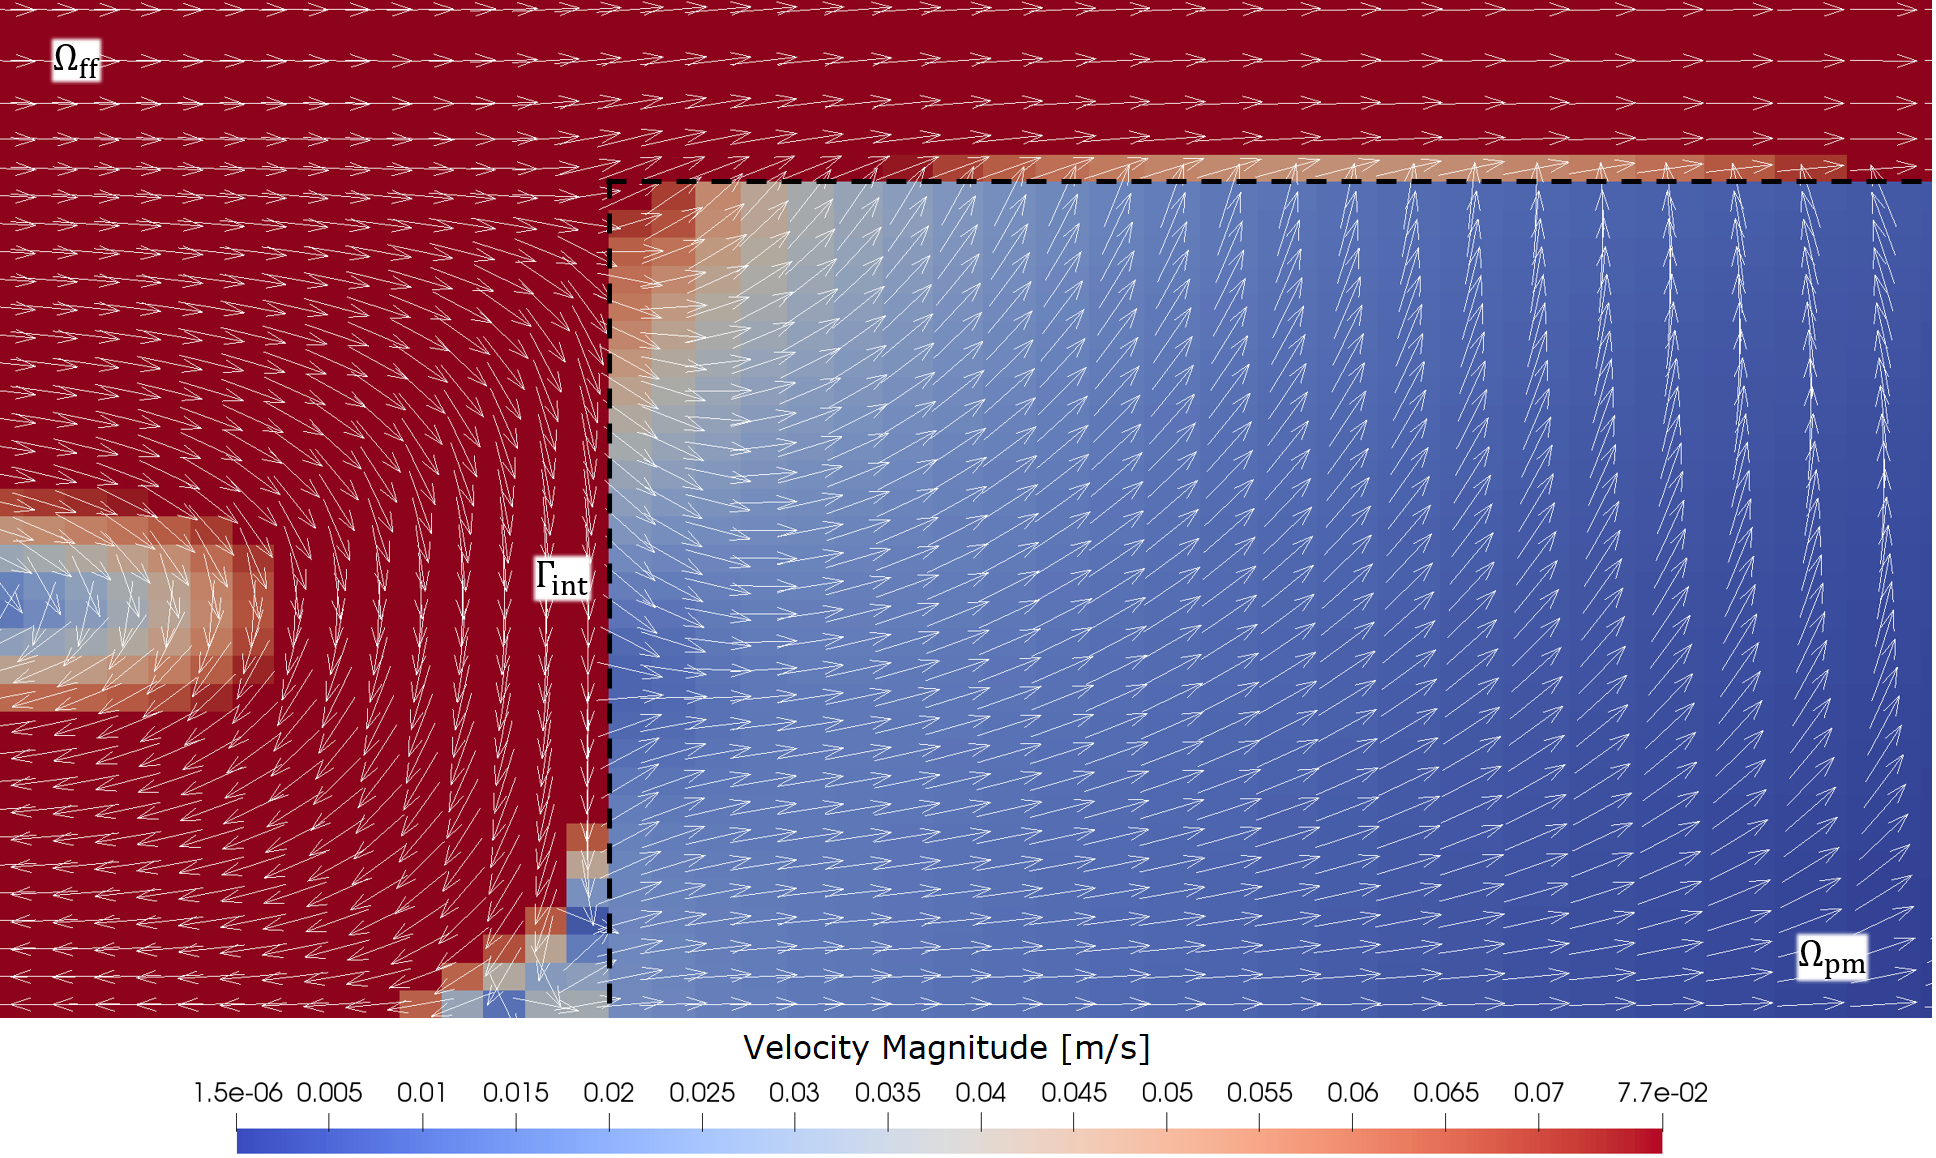
\includegraphics[height=0.8\textheight]{coupled_first_cavity_slides_labels.png}
	\caption{\tiny $\mathrm{K}=\SI{3.1e-7}{m^2}$, $Re=\num{6e5}$}
\end{figure}
\end{frame}
%%%%%%%%%%%%%%%%%%%%%%%%%%%%%%%%%%%%%%%%%%%%%%%%%%%%%%%%%%%%%%%%%%%%%%%%%%%
\begin{frame}{Coupled problem with shallow cavities}
\begin{figure}
	\centering
	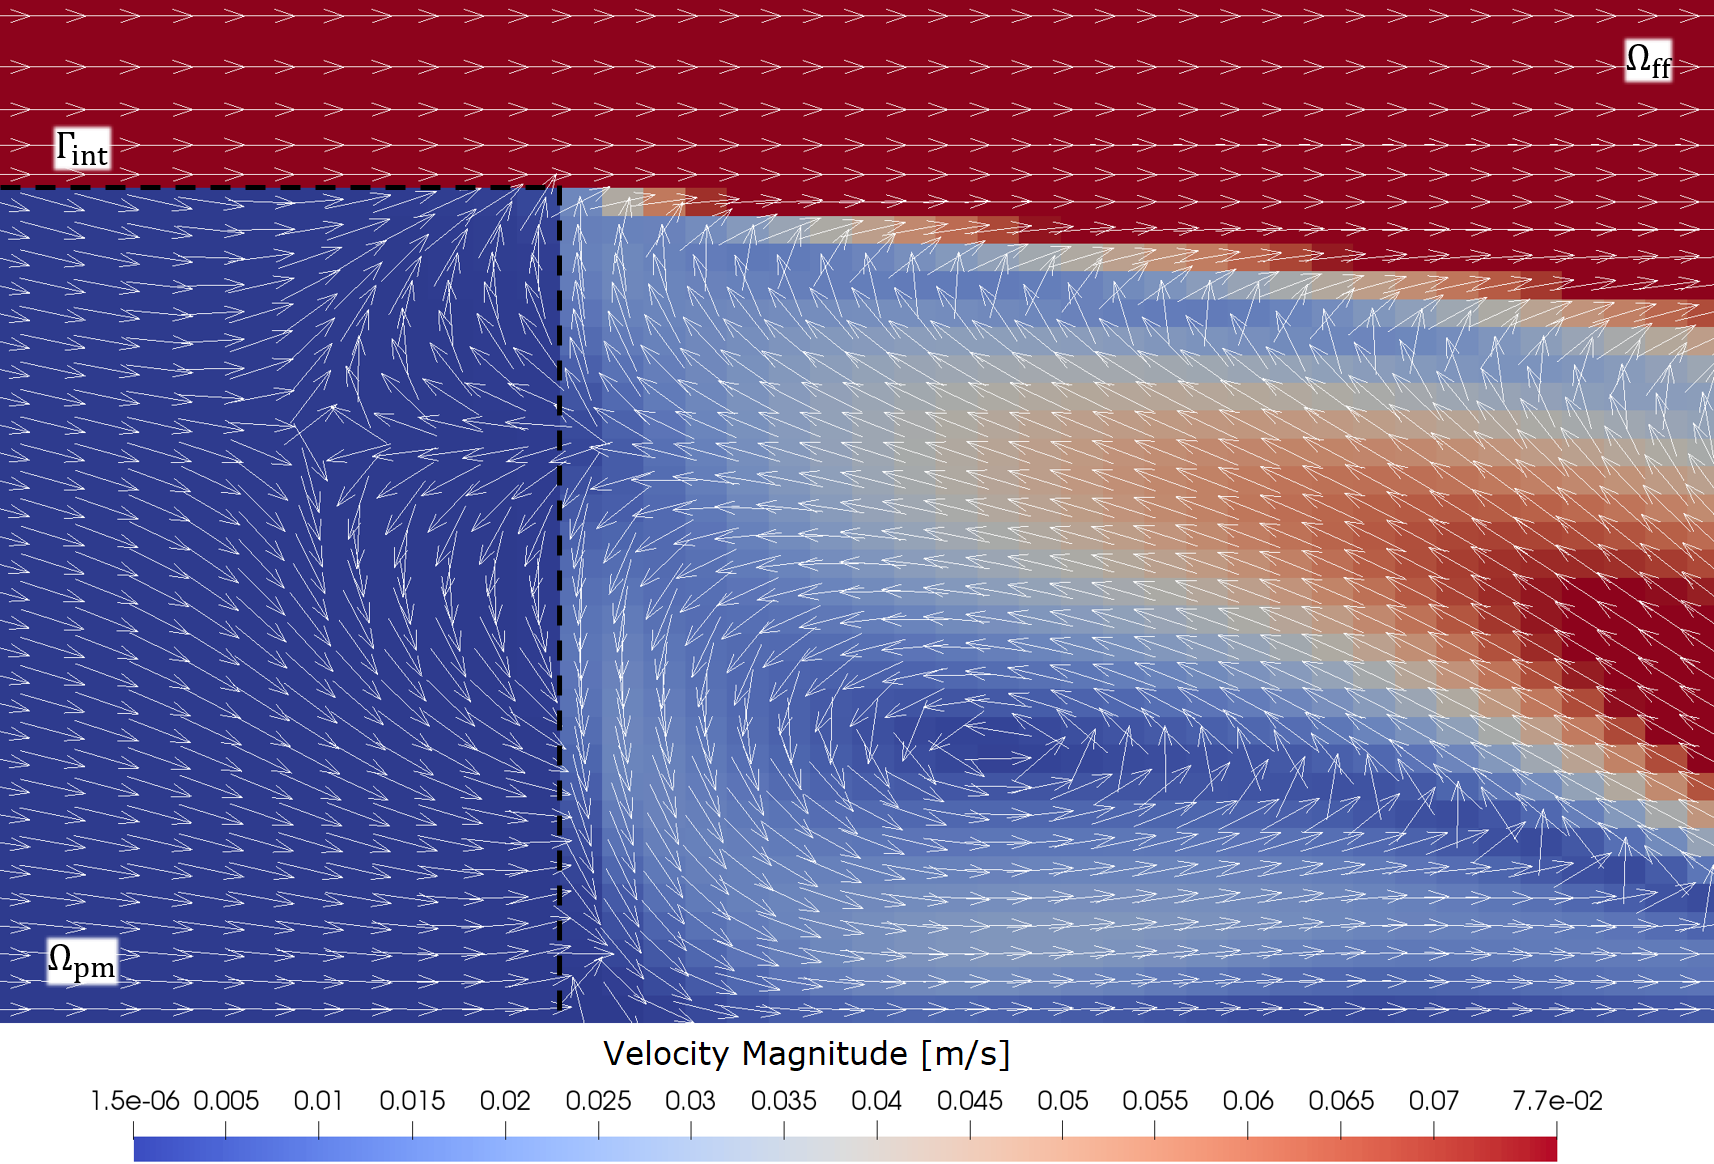
\includegraphics[height=0.82\textheight]{coupled_second_cavity_slides_labels.png}
	\caption{\tiny $\mathrm{K}=\SI{3.1e-7}{m^2}$, $Re=\num{6e5}$}
\end{figure}
\end{frame}
%%%%%%%%%%%%%%%%%%%%%%%%%%%%%%%
\begin{frame}{Coupled problem with cavities}
\textbf{Mass flow rate} $[\si{kg/s}]$ from the free-flow region to the porous-medium across $\Gamma_\text{int}$.
\begin{columns}
	\column{0.4\textwidth}
	\begin{equation*}
	\dot{m} = \int_{\Gamma_\text{int}} \max \{ \varrho \mathbf{v} \cdot 
	\mathbf{n}_\text{ff} , 0 \} \; dA
	\end{equation*}
	\column{0.6\textwidth}
	\begin{figure}
		\centering
		% This file was created by matlab2tikz.
%
\definecolor{mycolor1}{rgb}{0.00000,0.44700,0.74100}%
\definecolor{mycolor2}{rgb}{0.85000,0.32500,0.09800}%

\begin{tikzpicture}

\begin{axis}[%
width=1.05\widthsette,
%width=0.951\widthsette,
height=0.95\widthsette,
at={(0\widthsette,0\widthsette)},
scale only axis,
xmode=log,
xmin=1e-12,
xmax=1e-05,
xlabel={$\mathrm{K} \; [\si{m^2}]$},
xlabel style={font=\scriptsize},
ymin=0.0005,
ymax=0.0045,
ylabel={$\dot{m} \; [\si{kg/s}]$},
ylabel style={font=\scriptsize},
axis background/.style={fill=white},
xmajorgrids,
ymajorgrids,
legend style={at={(0.03,0.97)}, anchor=north west, legend cell align=left, align=left, font=\tiny}
]
\addplot [color=mycolor1, line width=1.0pt, mark=o, mark options=solid]
  table[row sep=crcr]{%
3.1e-07	0.002690450574475\\
1.55e-07	0.00227104284972\\
3.1e-08	0.0013892852915599\\
3.1e-09	0.0007673545670522\\
3.1e-12	0.000648090673435001\\
};
\addlegendentry{Shallow cavities ($\SI{0.1}{m}$)}

\addplot [color=mycolor2, line width=1.0pt, mark=o, mark options=solid]
  table[row sep=crcr]{%
3.1e-07	0.00380516439666\\
1.55e-07	0.00306263879357\\
3.1e-08	0.001811656088526\\
3.1e-09	0.00108318452159\\
3.1e-12	0.000945936611289998\\
};
\addlegendentry{Deep cavities ($\SI{0.3}{m}$)}

\end{axis}
\end{tikzpicture}%
	\end{figure}
\end{columns}
\end{frame}
%%%%%%%%%%%%%%%%%%%%%%%%%%%%%%%%%%%%%%%%%%%%%%%%%%%%%%%%%%%%%%%%%%%%%%%%%%%
\section{Conclusions}
\begin{frame}{Conclusions}
TVD methods:
\begin{itemize}
	\item \textbf{improved accuracy}.
	\item improved prediction of the reattachment length in the backward facing step test.
\end{itemize}
Free-flow and porous-medium flow coupling:
\begin{itemize}
%	\item mutual influence of cavities.
	\item \textbf{permeability influence} on the flow field.
	\item mass flow rate.
\end{itemize}
%\pause
Outlook:
\begin{itemize}
	\item other kinds of roughness.
	\item more \textbf{complex scenarios} (non-isothermal, multiphase, etc).
	\item high order methods on adapted grid with hanging nodes.
\end{itemize}
\end{frame}
%%%%%%%%%%%%%%%%%%%%%%%%%%%%%%%%%%%%%%%%%%%%%%%%%%%%%%%%%%%%%%%%%%%%%
\begin{frame}{Main references}
\begin{itemize}
	\footnotesize
	\item T. Fetzer. `Coupled Free and Porous-Medium Flow Processes Affected by 
	Turbulence and Roughness'. PhD thesis. Universit\"at Stuttgart, 2018.
	\item J. Hou et al. `Improved total variation diminishing schemes for 
	advection simulation of arbitrary grids'. \emph{International Journal for 
		Numerical Methods in Fluids} 70 (2012).
	\item L. Li et al. `An improved r-factor algorithm for TVD schemes'. 
	\emph{International Journal of Heat and Mass Transfer} 51 (2008).
	\item K. Mosthaf. `Modeling and Analysis of Coupled  Porous-Medium and Free 
	Flow with Application to Evaporation Processes'. PhD thesis. Universit\"at 
	Stuttgart, 2014.
	\item D. A. Nield et al. \emph{Convection in Porous Media}. Springer, 2017.
	\item P. K. Sweby. `High Resolution Schemes Using Flux limiters for 
	Hyperbolic Conservation Laws'. \emph{SIAM Journal on Numerical Analysis} 
	21(5) (1984).
	\item H. K. Versteeg et al. \emph{An Introduction to Computational Fluid 
		Dynamics: The Finite Volume Method}. Pearson Education Limited, 2007.
	\item D. C. Wilcox. \emph{Turbulence Modeling for CFD}. DCW industries, 
	2006. 
\end{itemize}
\end{frame}
\end{document}